
\documentclass[a4paper]{article}
%% Language and font encodings
\usepackage[english]{babel}
\usepackage[utf8x]{inputenc}
\usepackage[T1]{fontenc}

\usepackage[authoryear]{natbib}
\usepackage{subcaption}
%%  \usepackage{subfig}

%% Sets page size and margins
\usepackage[a4paper,top=3cm,bottom=2cm,left=3cm,right=3cm,marginparwidth=1.75cm]{geometry}

%% Useful packages
\usepackage{amsmath}
\usepackage{graphicx}
%\usepackage[colorinlistoftodos]{todonotes}
\usepackage[colorlinks=true, allcolors=blue]{hyperref}

%% My definition
\newcommand{\toshi}{\textcolor{blue}}
\newcommand{\laurie}{\textcolor{red}}
\newcommand{\rishi}{\textcolor{green}}
\newcommand{\iago}{\textcolor{purple}}

\usepackage{algorithm}
\usepackage{algorithmicx}
\usepackage{algpseudocode}

\title{Stock assessment grids: or why being lazy is a sign of intelligence.}
\author{Laurie Kell, Iago Mosqueira, Henning Winker, \\Rishi Sharma, Toshihide  Kitakado, Max Cardinale}

\begin{document}

\maketitle

Dear All

This is the old "VPA" problem, and demonstrates the need for validation, is a reason for MSE, and illustrates the difficulty with finding a "best" assessment.

In VPA there is little information to estimate incoming year classes, i.e. recruitment or F/selectivity. Therefore shrinkage is often used to reduce variability in terminal year estimates. This was driven by a need to reduce retrospective patterns, a main criteria for acceptance of an assessment in ICES. To do this often shrinkage is used.  In statistics shrinkage is used to reduce variance at the expense of bias. Using model based quantities, however, means that in a retrospective analysis bias is unknown.  Therefore the easiest way to get rid of a retrospective pattern is to ignore the data! That is why to validate a model you must use observations to validate prediction skill.

An implicit lack of prediction skill is recognised by management frameworks, since many stocks are assessed annually and management adjusted as required. Or in other words feedback is used. MSE is a formal way of modelling feedback. The next issue with MSE is conditioning Operating Models, and a key issue is the observation error model and when conditioning OMs MASE should be used to identify indices with good prediction skill.



Henning,
Such a study on role of composition data in recruitment process estimation would be helpful.

When there is moderate process error in recruitment (sigmaR >0.5) and the composition data are moderately informative (effective N 25-50) and Z<0.5, then I find that during historical years the composition data are highly informative about recruitment because their information content reinforces across years to measure cohort strength.  But at the end of the time series, the composition data cannot reinforce across years so the model tendency is to estimate spuriously high/low recdevs to match the data. So, I think there may be a need for a new model control that reduces input N for composition data near end of the time series such that the sigmaR penalty dominates and recdevs then stay closer to 0.0.

But that raises a bigger issue: what should the expected recruitment be near the end of the time series. This is especially problematic for assessments that use a fixed steepness value and do not use autocorrelation in recdevs.  These models force the ending year and forecast recruitments to by highly determined by model structure and not by data.  There should be a way to guide the ending years/forecast recruitments to be closer to well-estimated preceding recruitments.



\begin{abstract}

%The adoption of the Precautionary Approach to fisheries management requires a formal consideration of uncertainty. In the stock assessment process uncertainty about resource dynamics are commonly represented by alternative model structure, datasets and parameters. The use of integrated assessment models has meant that fitting to all available data has become commonplace as scientists seek to use the models to capture all knowledge about stock size and productivity. Therefore, ensembles of models are increasingly being implemented with scenarios based on fixing hard to estimate parameters, and to explore data weighting. The same approach is sued for conditioning Operating Models for use in Management Startegy Evaluation. Key questions to answer in both cases is does the model fit the data, are the resource dynamics plausible, and are the results robust. 

\end{abstract}

\newpage
\subsection*{Introduction}

The adoption of the Precautionary Approach to fisheries management \citep[PA,][]{garcia1996precautionary} requires that undesirable outcomes be anticipated and measures taken to reduce risk. Where risk is an uncertainty that, if it occurs, will have an effect on management objectives, which in the case of scientific fishery management frameworks are to provide the basis for long-term sustainability. Stock assessment therefore, requires making and validating probabilistic estimates of stock status and forecasts of the consequences of management actions relative to target and limit reference points. This, requires as well as considering statistical uncertainty taking into account incomplete knowledge about stock dynamics, observation processes, the effects of environmental variability, the behaviour of the harvesting sector, and managers ability to monitor and change exploitation levels. There are three main ways of considering uncertainty in stock assessment; the use of integrated statistical models, combining outputs from multiple models, and conducting Management Strategy Evaluation (MSE).

Integrated analysis combines several sources of data into a single model by a joint likelihood \citep[e.g][]{maunder2013review}. Many important process which impact estimates of quantities of management interest, however, may be misspecified and result in data conflicts \citep{carvalho2017can}. Common solutions are to develop alternative models with different assumptions and structures and to down weighted or eliminated conflicting data.  The different scenarios then need to be validated \citep[e.g.][]{kell2020validation}. Validation, however, is not a binary proces, i.e. pass or fail, as models often represent a continuum between these extremes. This means that it is not always possible to choose a "best assessment", and instead results from multiple models are combined \citep{brodziak2005model} for example in the advice framework of the tuna Regional Fisheries Management Organisations \citep[RFMOs][]{kell2016quantification}. When combining multiple models parameter estimates are usually intermediate to those obtained from the individual models. However, the most likely parameter values may not be intermediary but occur at one of the apparent extremes \citep{schnute1993analysis}. 

The choice and weighting of scenarios therefore has consequences for advice as often divergent views and beliefs mean that uncertainties can be used to support stakeholder positions in order to strengthen or weaken management measures \citep{fromentin2014spectre}. In addition management frameworks stock indicators are permitted to fluctuate around targets but limits should not be breached, this means that the distributions of derived estimates are important. For example to achieve Marine Stewardship Council (MSC) certification, there need to be at least a 50\% probability of being above a biomass and below a fishing mortality target, but at least a 95\% probability of avoiding a limit. %The choice and weighting of stock assessment scenarios can therefore have economic consequences since if a fishery achieves MSC certification there is a price premium. 

%This is the old "VPA" problem, and demonstrates the need for validation, is a reason for MSE, and illustrates the difficulty with finding a "best" assessment. In VPA there is little information to estimate incoming year classes, i.e. recruitment or F/selectivity. Therefore shrinkage is often used to reduce variability in terminal year estimates. This was driven by a need to reduce retrospective patterns, a main criteria for acceptance of an assessment in ICES. To do this often shrinkage is used.  In statistics shrinkage is used to reduce variance at the expense of bias. Using model based quantities, however, means that in a retrospective analysis bias is unknown.  Therefore the easiest way to get rid of a retrospective pattern is to ignore the data! That is why to validate a model you must use observations to validate prediction skill. An implicit lack of prediction skill is recognised by management frameworks, since many stocks are assessed annually and management adjusted as required. Or in other words feedback is used. MSE is a formal way of modelling feedback. The next issue with MSE is conditioning Operating Models, and a key issue is the observation error model and when conditioning OMs MASE should be used to identify indices with good prediction skill.


The ability of stock stock assessment models to make long-term projections is generally poor, therefore many stocks are assessed annually and management adjusted as required. Or in other words feedback is used where information about the difference between the current and a reference level is used to alter the gap \citep{ramaprasad1983definition}. MSE is a formal way of modelling feedback. When conducting MSE a set of operating models (OMs) are conditioned on data and knowledge to represent hypothesis about resource status and dynamics. A common way to condition OMs is by fitting an integrated assessment model to the available data \citep{sharma2020trfmo}. The OMs are then used to evaluate the performance of strategies modelled as Management Procedures (MPs), the combination of monitoring data, analysis method, reference points, harvest control rule and management measure. MPs act as feedback controllers, the aim of which is to keep the state of the system within agreed bounds despite uncertainty about system dynamics. This negates the need to find a "best assessment", as the MP may be a black box with no knowledge of the assumed processes, requiring only knowledge about the behavior of the system. 

An aim of conditioning an OM, like stock assessment, is to reject models that do not fit the data satisfactorily and are consequently inconsistent with the actual situation observed. The intention is not to find a "best assessment" but to agree a limited set of OMs with high plausibility, that include the most important uncertainties in the model structure, parameters, and data. A definition of a highly plausible scenario is one that fits prior knowledge well: with many different sources of corroboration, without complexity of explanation, and with minimal conjecture \citep{Connell2006model}. Plausibility may be estimated formally based on a statistical approach, or specified based on expert judgement, and can be used to weight performance across summary statistics related to yield and sustainability when integrating over results for different OM scenarios representing alternative hypotheses. Alternatively rather than weighting a large number of scenarios, to be acceptable a strategy must perform well across all scenarios that pass a selection criteria. 
%Where performance is based on statistics which ideally should be few, informative and with axes related to status, safety, yield, and stability. 
In either case the choice of the OMs and weighting schemes are critical %since performance statistics is therefore key, since once agreed the best management strategy is an emergent property.  Therefore open and transparent procedure for agreeing and weighting OMs is crucial in order to increase trust. 

Although OMs are commonly conditioned by fitting an integrated assessment model, there are concerns about the use of such models due to a lack of transparency because of the many internal, implicit and often poorly documented assumptions, and a lack of access as only a few highly skilled modellers can run such complex models \citep{hilborn2003state}. Paradoxically, a reason for MSE was to move away from complex assessment models in order to provide more access and to develop simple rules that could be better understood by stakeholders. 

As the number of assessment and operating model scenarios increase advice depends on the models selected and weights given to the different models when post processing. In all cases model validation and clear and transparent communication of model results is required to increase confidence amongst the public, stake and asset-holders, managers and policymakers \citep[][]{saltelli2020five}. We therefore investigate the use of different procedures for weighting models by revisiting the OMs of the Indian Ocean Albacore MSE. THe OMs were conditioned using an integrated stock assessment and a factorial design to consider the main uncertainties. We use this grid as a worked example and discuss the consequences for choosing a best assessment, ensemble modelling, and conducting MSE, of different ways for selecting models and assigning weights. We review what we did given tRFMO recommendations and recent work on model diagnostics and ensemble modelling. Testing the approach on an actual case study first was informative as it provides the insight necessary to set up a study on synthetic data. 

\section*{Material and Methods}

Selection and weighting criteria fall into three categories i) expert opinion; ii) goodness of fit; and iii) plausibility. A variety of metrics have been proposed for weighting or ranking models e.g. based on convergence, likelihood, AIC, RMSE, runs tests, retrospective analysis, hindcasting and prediction skill. It is also important to adopt an objective approach to selecting and weighting models in order to overcome artifacts and biases introduced by a hand-picking approach \citep{pechlivanidis2018information}. When choosing metrics the total number should be minimised, complementary and non-redundant \citep{shin2010can, kershner2011selecting}. This is because results are sensitive to the choice of attributes, the methods used in their derivation, the weights applied when combining them. For example random errors may lead to a switch in relative weights and rankings, and so influence outcomes considerably \citep{freyer2014robust}. Robust rankings, where ranking order is stable, are normally considered to be reliable and trustworthy, and conversely non-robust rankings as unreliable and unstable \citep{permanyer2011assessing}. The robustness of ranking in a composite metric, however, may be due to a redundancy of attributes. Robustness can therefore be both desirable and undesirable simultaneously. It also makes little sense to combine correlated metrics
\citep{mcgillivray1991human} as weighting should consider the information content within the models, it is better therefore to identify the key attributes and weight accordingly.

\subsection*{Material}

An Operating Model for the albacore tuna (\textit{Thunnus alalunga}) fishery and stock in the Indian Ocean has been developed by the Indian Ocean Tuna Commission (IOTC) to evaluate the performance of alternative Management Procedures (MPs). The operating model was conditioned using stock synthesis \citep[SS3][]{MethotW2013} based on the current best knowledge and data \citep{ptmt2014}. Datasets include records of catches and landings, indices of abundance based on catch per unit (CPUE), and  saamples of length and ages compositions. Reformulating model structure, however, is time consuming and so scenarios were based on the choice of parameters for which there is insufficient information in the data to estimate and data weighting. 

The assessment partitions the Indian Ocean into four regions, divided latitudinally along the 25$^{\circ}$S parallel and longitudinally along the 75$^{\circ}$E meridian, 
 figure \ref{fig:map} show the distribution of catches. The assessment includes a total of 11 fisheries, including  aggregated Longline fishery for each of the four regions  \citep{LangleyH2016}, and a set of standardised CPUE indices has been derived from longline catch and effort data provided by Japan, Korea and Taiwan, China. \citep{HoyleKL2016} (Figure \ref{fig:u}). Area 3 is considered to represent the core of the distribution of the stock.

Fisheries dependent data is in general less informative that would be ideal for estimating a large number of confounded model parameters. In the case of the Indian Ocean albacore stock, a number of reasons limit the ability to obtain reliable model fits. Problems exists with the data completeness and quality \citep{IOTC2016WPTmT0607}, not limited to but including total catch statistics, length distribution in catches, and biological information. The main factors currently considered in the structural uncertainty grid for the albacore OM are shown in  table \ref{tab:om})


\subsection*{Methods}

The operating model was conditioned using stock synthesis \parencite[SS,][]{methot2013stock} which  implements an age and spatially structured model that reflects the complex population and fishery dynamics of the stock. 
%There has been a recent trend in stock assessment toward the use of integrated analysis that combines several sources of data into a single model by a joint likelihood for the observed data \parencite[e.g.][]{doubleday1976least,fournier1982general,maunder2013review}. data sets include records of catches and landings, indices of abundance based on catch per unit (CPUE) or from research surveys, and length and age compositions based on samples. An example of an integrated assessment method is SS that can be configured in multiple ways, allowing for a range of scenarios to be developed to reflect uncertainty.

The base case considered in the stock assessment session was then extended by considering factors with levels intended as a sensitivity analysis. There included i) alternative values of natural mortality (M) for juveniles (ages 0 to 4) and adults (age 5 or older); ii) two values for the variability of recruitment in the population (sigmaR) of 0.4 and 0.6; iii) three values for the steepness ($h$) of the stock-recruitment relationship 0.7, 0.8, and 0.9; iv) four values for the coefficient of variation in the CPUE series of 0.2, 0.3, 0.4 and 0.5; v) three values for the relative weight of length sampling data in the total likelihood, through changes in the effective sampling size parameter, of 20, 50 and 100; vi) two scenarios for the effective catchability of the CPUE fleet: it was assumed that the fleet had not improved its ability plus an alternative scenario that considered a 2.5\% increase in catchability; vii) two possible functional forms for the selectivity of the CPUE LL fleet were considered: a logistic function (Log), where selectivity stays at the maximum level, or double normal (DoNorm), where selectivity drops at some point in the age range.


\subsubsection*{Estimation Error}

Observation uncertainty is related to parameter uncertainty as the parameters are estimated from the observations and the variance assumed for the observations dictates the parameter uncertainty.

High assessment uncertainty can indicate a lack of contrast in  the input data or violation of model assumptions.


Estimation error was generating using a delta-multivatiare lognormal approach (delta-MVLN). This takes the means and variance-covariance matrix of $log(SSB/SSB_{MSY})$ and $log(F/F_{MSY})$. Let $u = SSB/SSB_{MSY}$ and $v = F/F_{MSY}$  and $x = log(u)$ and $y = log(v)$ , then the $VCM$ has the form:
    			
\begin{equation}
VCM_{x,y} =
\begin{pmatrix}
\sigma^2_x & cov_{x,y}  \\
cov_{x,y} & \sigma^2_y
\end{pmatrix}
\end{equation*}

\noindent 
where  is the variance of x,  is the covariance of y and  is the covariance of x and y.  The quantities that can be directly extracted from Stock Synthesis are: (1) MLEs, asymptotic standard errors (SE) and correlation of $SSB/SSB_{MSY}$  and $F/F_{MSY}$. 
The construction of the  therefore requires to conduct a few normal to lognormal transformations. First, we approximate  and  as:

\begin{equation}
\sigma^2_x = \disp log\left(1+\left(\frac{SE_u}{u}\right)^2\right)  
\quad 
\end{equation}

and

\begin{equation}
\sigma^2_x = \disp log\left(1+\left(\frac{SE_v}{v}\right)^2\right)  
\quad 
\end{equation}

\noindent where  and  is the asymptotic standard error estimate for $u = SSB/SSB_{MSY}$ and $v = F/F_{MSY}$. Second, the covariance of x and y can then be approximated on log-scale by:

\begin{equation}
COV_{x,y} = \disp log \right{1+ \rho_{u,v} \sqrt{\sigma^2_x\sigma^2_y}\right \quad 
\end{equation}

\noindent  where  denotes the correlation of u and v.
To generate the desired KPD for $SSB/SSB_{MSY}$  and $F/F_{MSY}$, we use a multivariate random generator, available in the R package ‘mvtnorm’, to obtain a large number (nsim = 10,000) of x and y pairs, such that

\begin{equation}
kobe_{x,y} = \disp MVN{\mu_{x,y},VCM_{x,y}) 
\quad 
\end{equation}

\noindent where  is the vector of the MLEs x and y. The joint MVLN distribution of $-SSB/SSB_{MSY}$  and $-F/F_{MSY}$ is then obtained as the exponential of $kone_{x,y}$.


\subsection*{Metrics}

\subsubsection*{Goodness-of-fit}

Analysis of residuals is a common way to determine a model’s goodness-of-fit \citep{Cox1968general}, since  non-random patterns in the residuals may indicate model misspecification, serial correlation in sampling/observation error, or heteroscedasticity. If the process of interest shows only random variation, the data points will be randomly distributed around the median. Random meaning that we cannot know if the next data point will fall above or below the median, but that the probability of each event is 50\%, and that the data points are independent. Independence means that the position of one data point does not influence the position of the next data point, that is, data are not auto-correlated. If the process shifts, these conditions are no longer true and patterns of non-random variation may be detected by statistical tests. Various statistics exist to evaluate residuals and nonparametric tests for randomness in a time-series include: the runs test, the sign test, the runs up and down test, the Mann-Kendall test, and Bartel’s rank test.

Non-random variation may present itself in several ways. If the process centre is shifting due to improvement or degradation we may observe unusually long runs of consecutive data points on the same side of the median or that the graph crosses the median unusually few times. The length of the longest run and the number of crossings in a random process are predictable within limits and depend on the total number of data points in the run chart \citep{anhoj2015diagnostic}.

A shift signal is present if any run of consecutive data points on the same side of the median is longer than the prediction limit, round(log2(n) + 3). Data points that fall on the median do not count, they do neither break nor contribute to the run \cite{schilling2012surprising}. A crossings signal is present if the number of times the graph crosses the median is smaller than the prediction limit, qbinom(0.05, n - 1, 0.5) \citep{chen2010impacts}. n is the number of useful data points, that is, data points that do not fall on the median. The shift and the crossings signals are based on a false positive signal rate around 5\% and have proven useful in practice.

\subsubsection*{Model based prediction skill}

In a retrospective analysis observations are sequentially removed from the terminal year backwards (i.e. peeled), the model is then refitted to the truncated series and model estimates compared to see if there are any systematic patterns. Mohn's $\rho$ \parencite{mohn1999retrospective}, is commonly used as a measure of relative error. We use a variant scaled by the mean so the metric is not affected by the length of the peel or the number of step aheads.

\begin{equation}
\label{eqn:mohn}
\rho_{M} = \disp \frac{1}{n} \sum_{t=T-n}^{T-1} \frac{\hat{y}_{(1:t),t}-\hat{y}_{(1:T),t}}{\hat{y}_{(1:T),t}} 
\end{equation}

\noindent
where , $n$ is the number of time steps that the peel is performed for, $t$ is the time for which the missing value is being estimated, $T$ is the terminal year in the time series, and $\hat{y}$ denotes a model based quantity. The value with suffix $\hat{y}_{(1:T)|t}$ means a value estimated at time $t$ from the full series running from time 1 to $T$, and $\hat{y}_{(1:t),t}$ is the value estimated using the data window from 1 to $t (\leq T)$. 

$\rho_M$ is an average of the relative differences at the final time of each window, and is a measure of relative retrospective `bias' (scale-free) in a statistical sense. The metric tends to be applied not on the log but the original scale because both the directions of positive and negative bias are regarded as being equivalent. $\rho$ can be estimated for different horizons 
\begin{equation}
\label{eqn:mohn}
\rho_{M} = \disp \frac{1}{n-h+1} \sum_{t=T-n}^{T-h} \frac{\hat{y}_{(1:t)|t+h}-\hat{y}_{(1:T)|t+h}}{\hat{y}_{(1:T)|t+h}} 
\end{equation}

For reference values which are low relative to the alternative there is no upper limit, while in the reverse case the error cannot exceed 1.0. Therefore, in practice its usual to use a lower bound of -0.15 and an upper bound of 0.20 to identify acceptable performance \parencite{hurtado2014looking}. For values near or equal to 0, e.g. stocks where exploitation or stock size is low, small absolute differences can result in large relative differences.  This may result in assessments being rejected when they are needed the most, e.g. during the development of recovery plans, when both stock biomass and fishing mortality may be low. 

\subsubsection*{Model free prediction skill}

Validation, requires that the system be observable and measurable and so model free quantities should be used, unless model estimates are known to be very close to their true values. In stock assessment, however, bias is difficult to quantify. For example a reduction in mean squared error (a measure of variance) can be achieved by shrinkage at the expense of prediction skill. The absence of retrospective patterns in model based quantities, therefore, while reassuring is not sufficient for validation. Validation should therefore be conducted using prediction skill based on observations. We therefore used the models to generate pseudo data based on CPUE and compare these to observations. 

Hindcasting involves fitting a model using a tail-cutting procedure, where data are deleted sequentially. This may be done for individual data series or combinations of different series, for example fleets where both CPUE and length data are removed. This allows data conflicts to be explored. Theoretically, the projection period is to the end of the historical time period, however, in practice, a step size of one or several years ahead (the horizon $h$) is chosen. This reflects the time horizon required for robust management advice; considering non-small process stochasticity in fishery population dynamics and non-ignorable extents of observation uncertainty. 

Assessment cycles are typically for three years in most tuna Regional Fisheries Management Organisations and so an horizon of three years was used.

Only CPUE observations were removed, catch and length composition remained in the model. Time series of pseudo data were generated from estimates of vulnerable biomass and catchability ($q$). Prediction residuals ($e$) were then computed as the difference between the predictions and the observations. 

Prediction skill based on a forecast compares an observation at time $t$ ($y_t$) to an estimate of that observation made $h$ time steps previously ($\hat{y}_{t|t-h}$). To do this we use the mean absolute scaled error (MASE), as it is a robust and easy to interpret statistic \parencite{hyndman2006another}. The MASE compares prediction error ($e_t$) for a prediction horizon of $h$ 

\begin{equation}
\label{eqn:skill}
 e_t = y_t -\hat{y}_{t|t-h} 
\end{equation}

\noindent 
to a benchmark forecast corresponding to a na\"{i}ve forecast equal to the last observed value. 

\begin{equation} 
{\hat {y}}_{t|t-h}=y_{t-h}}
\end{equation}

\noindent For a peel of $n$ and a horizon of $h$ years

\begin{equation}
\label{eqn:skill}
\eqn{MASE={\frac {\frac{1}{n+1}   
\sum _{t=T-n}^{T}\left|y_t - \hat{y}_{t|t-h}\right|}{
                  \frac{1}{n+1+h} 
                  \sum _{t=T-n-h}^{T}\left|{y_{t} - {y}}_{t-h}}\right|}}} \\
\end{equation}

The MASE has the desirable properties of scale in-variance so can be used to compare forecasts across data sets with different scales, predictable behaviour, symmetry, interpretability and asymptotic normality. Unlike relative error MASE does not skew its distribution even when the observed values are close to zero, is easy to interpret as a score of 0.5 indicates that the model forecasts are twice as accurate as a na\''{i}ve baseline prediction. The Diebold-Mariano test \parencite{diebold1995comparing} for one-step forecasts can also be used to test the statistical significance of the difference between two sets of forecasts. 

\subsubsection*{P-values}

The relationship between Mohn's $\rho$, $-2log(p)$ for the runs test and MASE is summarised in figure \ref{fig:xxx}. A high value of a combine p-value and $\rho$ shows that both metrics are in agreement, and since $\rho<0.2$ that the tests are favourable. For example inspection of the "good" scenarios in pink shows that the fit is good but there is poorer prediction skill overall.

\newpage
\section*{Results}

Time series of catch, and spawning stock biomass and fishing mortality relative to $MSY$ target reference points are shown in figure \ref{fig:ts}, for the base case (black line) and the main effects. Catches started to increase in the 1950s, and have varied just above $MSY$ in in the last two decades. Fishing has resulted in $SSB$ declining but it is still estimated to be above $SSB_{MSY}$ in all but one scenario, while $F$ is increasing and is above $F_{MSY}$ in around half of the scenarios.

The expected dynamics are summarised, for the main features across all scenarios in the form of production functions in figure \ref{fig:pf}; rows correspond to the steepness of the stock recruitment relationship, columns to natural mortality of adults, and colours to ESS. The main features are a change in the shape of the production as natural mortality increased for adults and a reduction in scale as with effective sample size. Scale and the ratio between $SSB_{MSY}$ and virgin biomass decreases with steepness, although the effect is less pronounced that for M and ESS. Juvenile natural mortality had no effect as catches are mainly of adults. The increase in adult natural mortality results in the stock becoming more robust to exploitation; since to explain the catches the stock most be more productive, as seen by the increase of the slope at the origin, and hence population growth rate ($r$).   

Kobe phase plots are used by the tuna RFMOs to make statements of probability about stock status relative to target $MSY$ reference points. Figure \ref{fig:kobe} shows $SSB/B_{MSY}$ and $F/F_MSY$ in the terminal year for the main effects with estimation error (cyan points denote the median, figure \ref{fig:kobe-main}) and for the base case with estimation error and model error (figure \ref{fig:kobe-bg}). Only 1 main effects (M0202?) is in the red quadrant ($SSB > SSB_{MSY}$ and $F < F_{MSY}$), i.e. there is only a probability of $7\%$ of the stock being overfished and subject to overfishing when model error is considered. When a best assessment and estimation error is considered there is a X\% chance of being in the red quadrant, which increases to Y\% when all main effects and estimation are considered, and to Z\% when all only model error is considered. \red{This shows that uncertainty is underestimated if only estimation error is considered, implies over-fitting and a reduction in variance at the expense of bias. It must be noted, however, that estimation error was generated by the delta-MVLN approach, and not by the bootstrap or the jackknife so the the median of estimation error and the fit are the same and bias is not shown.} 

The fits are summarised by the runs test, the number of expected crossing (\refl{fig:runs}) and prediction skill by MASE (\ref{fig:mase}), and the log likelihoods, AIC and number of parameters are shown in figure \ref{fig:aic}.
  
A major diagnostic for acceptance for acceptance of an assessment is Mohn's $\rho$ and Figure \ref{fig:mohn-1} summarises the 1-step ahead model-based predictions for $SSB$ and Figure \ref{fig:mohn} the 3-step ahead projections. Main effects are indicated by the vertical lines. Over half of the main effects fail the Mohn's $\rho$ test. The distribution  is bi-modality with one mode centred on 0, i.e. some scenarios show little bias. The main effect and base case, however are centred around the lefthand mode. As the time step increases more scenarios fall below the Mohn's $\rho$ threshold of -0.15. Figures \ref{fig:mohn-1-corner} and \ref{fig:mohn-corner} show the same value of Mohn's $\rho$ but this time the vertical lines show the corners of the grid.

%Figure \ref{fig:runs} therefore compares the runs tests based on the model residuals to the prediction residuals for the entire grid. The number of crossings (figure \ref{fig:runs-cross}) and the length of the longest run (figure \ref{fig:runs-long} and the MASE (figure \ref{fig:mase}). Most of the scenarios and indices pass the crossings test, while performance for the length of the longest run is poorer. Indices 2 and 3 perform best. The value of Mohn's $\rho$ does not appear to have an impact. 
   
%\item The results for MASE from the model-free hindcast are different from the runs tests, in that Mohn's $\rho$ does appera to have an effect, i.e. a scenario and index has a value of $MASE \gt 1$ it also tends to have lower prediction skill.  While the relative performance of indices 2 and 3 is similar to the runs tests, index 4 now has good performance.
   
%\item The p-values by scenarios for MASE and the runs test are compared to Mohn's $\rho$ in figure \ref{fig:wts}. These show that in the sceanrios with good prediction skill indices perform better, based on MASE. The runs test does not appear to be an indicator of prediction skill, potentially due to overfitting. 

A regression tree was used to identified the factors that influence Mohn's $\rho$ for the 3-step ahead procedure (figure \ref{fig:tree}). The corresponding time series of SSB (\ref{fig:tree-b}), production functions (\ref{fig:tree-pf}), and time series of surplus production (\ref{fig:tree-sp}), i.e. the emergent properties, are also summarised. The first split is on natural mortality of the adults, if this is $< 0.4$ then the test that Mohn's $\rho > -0.15$  is passed (red). The two exceptions are for M=0.3 and CPUE CV = 0.2 or 0.3 which fails  and M=0.4 and CPUE CV = 0.5 \& ESS = 100 which passes. In other word the biggest impact is M, and high M is only plausible when the CPUE are down weighted compared to the length data. The more plausible dynamics are for lower values of biomass, $MSY$, and $SSB_{MSY}$ and less variability in productivity.

The different metrics are compared in figure \ref{fig:xxx}, Mohn's $\rho$ and the goodness of fit diagnostics (cross, long, and p.runs) are correlated, while MASE (p and n) are negatively correllated. Weighted phase plots for targets and limits are presented in figure \ref{fig:phase-wt} for equal, simple skill based, and AIC weighting. If the Mohn's $\rho$ test is used to select and reject scenarios the stock is overfished. AIC has little impact.

Table \ref{tab:smry} summarises the risks of overfishing and being overfished, while table \ref{tab:smry2} summarises the risj of the stock breaching the biomass limit reference point. 

   %\item Developing an Observation error model is also a part of conditioning an operating model. Therefore figure \ref{fig:mase} shows the indices of abundance (\ref{fig:mase-u}) and their values of MASE (\ref{fig:mase-score}). Many of the indices have gaps or do not cover the entire period and so were not considered. Of the remaining indices index 3 for quarters 2 and 3 were considered as these cover the main area of distribution of the stock and had the best values of MASE for all indices \item Figure \ref{fig:xxx}.
   
   %\item Figure \ref{fig:xxx} shows the relationship between MASE and Mohn's $\rho$, broken up by $M$. The bimodality is driven by M, i.e. MASE increases with M of adults. To explore the impact of bias in the index the results were also broken out by catchability; MASE  improves if a trend in catchability is assumed. 
   
  
  %\item Figure \ref{ref:grid} summarises a variety of summary metrics by adult M and steepness for Mohn's $\rho$. $SSB/B_{MSY}$ (\ref{fig:grid-bmsy}), $B_{lim}$ (\ref{fig:grid-blim}), $F/F_{MSY}$ (\ref{fig:grid-fmsy}), $r$ (\ref{fig:grid-r}), $K$, (\ref{fig:grid-k}), $p$, (\ref{fig:grid-p}), $sd(sp)$, (\ref{fig:grid-sp}), and Population doubling time (\ref{fig:grid-dt}). There is some modality due to catchability, particulary in current biomass status and $K$.  Again the biggest impact is adult M. 

\end{itemize}

\newpage

\section*{Discussion}

Estimating prediction skill showed that alternative models were equally well able to explain the data, which in turn explains why estimation error was less than model error. In consequence if the objective had been to select a best assessment, uncertainty and hence the risks, e.g. of the stock being overfished or of foregoing yield, may have been underestimated. Therefore the hindcast procedure was used to weight a multi-model ensembles using skill-based weighting (SW), and compared to equal weighting (EW), and AIC weighting. The prediction skill score was used to assign more weight on the better performing models as this has been found to improve forecasts \parencite[e.g.][]{casanova2009weighting}. This can be done to weight estimates of current status relative to reference points, as here, or to weight operating models.

The initial choice of scenarios and metrics for post processing had a big effect on estimates of stock status relative to reference points. If EW is used the stock is ?? while if SW based on model-based quantities it is ??? and ??? for model-free.  While the outcome of AIC weighting depends solely on the choice of ESS. There were significant correlations between some potential weighting metrics (e.g. between Mohn's $\rho$ for model based quantities and the p-value for the runs test), suggesting these metrics are proxies for the same property, and if both had been used for weighting would have given this property twice the weight. A potential explanation is that if an influential index showed a systematic residual pattern in the recent period and then a hindcast was performed then it is like to have a large value of Mohn's $\rho$ and a large p-value. In contrast the metrics for the model free hindcast was negatively correlated. This could be due to the interaction with ESS, since as ESS increased so did goodness of fit resulting in a reduction in prediction skill of the CPUE indices.

The use of feedback relaxes requirement for prediction skill. Feedback, i.e. where management action seeks to respond to changes in system state and readjust the control accordingly, does not require great prediction skill. For example it was shown that Mohn's $\rho$ was better for a 1-year than a 3 year step ahead, i.e. the ability to assess the consequences of management 1 year head is is better than the ability to assess the consequences 3 years ahead. Therefore to ensure limits are not breached a 1 year assessment cycle may perform better than a three year cycle. There may be a trade-off, however, in inter-annual catch variability and an associated cost. This can be evaluated using MSE. However, the results of MSE will depend on the choice of scenarios.    
    
Where it is thought desirable to “condition” OMs by fitting to the available data to ensure that they are compatible with the information, compatibility needs to be checked by examining standard model diagnostics. In particular, if indications of model misspecification are evident, the model needs to be rejected, or at minimum assumptions re-examined. Such checks can be difficult to conduct thoroughly however, when a large number of OMs are under consideration. Also an important use of MSE is to identify where improvements to data and knowledge can reduce risk. This requires OM scenarios that allow resolving uncertainty to be evaluated, i.e. what if measurement error was reduced by improved sampling, to do this can not be done using existing data alone as it requires simulation of alternative data sets.

A main issue with this worked example, was that the base case was not the "best" assessment, as it was worse, judged on Mohn's $\rho$, that any of the main effects. The cookbook approach, based on multiple tests and detours, could have been used to select a base case. The "best assessment" based on Mohn's $\rho$ was an interaction between M, CPUE and ESS. %Adopting the cookbook approach would hopefully help avoid the issue, seen in this case study, where it had a worse Mohn's $\rho$ than the main effects. This implies that the Base Case was incorrectly chosen, since if the Base Case had been run first it would have been rejected.
as shown by the regression tree showed. The main factor of importance was adult M, and the second was the relative weights of ESS and CPUE, i.e. fitting to stock trends or year-class variability and scale. Once a base case is selected then the main effects can be chosen. The cookbook with detours, however, is not appropriate since to be objective and transparent tests need to be pre-agreed and automated. A  rational for agreeing main effects and factors could be based for example on the IATTC approach for including models in an ensemble which is based on identifying the current issue with the stock assessment, then building models that fix these issues, typically by adding things that are usually not included in the base case model. This ideally should be done through a formal elicitation process to ensure engagement with stakeholders. Redundancy should be identified, i.e. five M scenarios were run (i.e. "0202", "0303", "0404", "0403", "0402"). The scenarios with M=0.4 for adults failed the Mohn's $\rho$ test, while juvenile M had no effect, as catches are mainly of adults. Therefore only 2 M scenarios are needed, i.e. "0202" and "0303". 

Once the impacts of potential main effects are identified, it is important to identify interactions. As shown in this case where the "best assessment" was an interaction. Crossing all the factors for the major uncertainties, especially if elicitation is used may result in a factorial increase in the number of scenarios. Efficiency may be improved by limiting scenarios to the “corner points”. For example for three factors each with three levels corresponds to a 3x3 cube, checks could be restricted to the 8 corner points rather than all 27 scenarios. If the results at the corners are satisfactory, it is not unreasonable to assume that the other OMs are satisfactory as well. If they are not, the range covered by the level choices for certain factors may need to be reduced until such a criterion is satisfied.

Using a limited number of OMs may be preferable to complex grid design, e.g. with the main effects only providing enough contrast for testing a MP against an OM, capturing only the most important uncertainties which are also the most influential as regards impact on management recommendations. A reason for this is because it is likely that it is the emergent properties, i.e. shape of the production function and the nature of the time series that will affect the performance of an MP. The regression tree showed that different assumed fixed parameters can produce the same features. It would therefore make sense to characterise the dynamics in the OMs, rather than exhaustically condition an integrated assessment on mltitudes of fixed parameters. In this case the dynamics were either high abundance and variability with most morality due to M, or low abundance and stable with most mortality due to fishing. In the later case the stock was overfished. 

^%Critically that are likely to beteria for as imporasessing the smaller grid design could be determined from sensitivity or elasticity analysis or from the base case variance-covariance matrix. Or by running a larger grid, and determining the main axis of uncertainty to estimate a smaller grid design using multivariate techniques. Starting with a smaller grid design (for a Reference Set of OMs) makes more practical sense, as it is difficult to check all diagnostics of all OMs run on a large grid. Less plausible or less influential uncertainties can be covered by robustness tests.
    
Very large sets of OMs should be avoided if possible, since checking all individual OMs is not practical, or even desirable even when tests are automated. A reason for this is because the MSE process unlike an ensemble is not trying to make probabilistic statements about stock status or forecast, but to identify strategies which are robust to uncertainty and where knowledge and data will reduce risk. A handful of OMs that reflect stakeholder concerns, and an objective transparent way of weighting performance measures based on OM scenarios is more useful that constructing an exhaustive grid. Since this will allow both the value-of-information and control to be identified. For example a lack of older fish in catches may be due to either higher M or reduced vulnerability of older individuals. The consequences for assessment and management will be different, improving the assessment requires more knowledge. While long-term fluctutions in stock biomass could be due to the environment or changes in vulnerability due to changes in distribution, in which case management based on size limits has been shown to be more robust that TAC \cite{fromentin2007consequences}.


    
        
\newpage
\section*{Conclusions}

\begin{description}
 \item[What we  did:]~ 
 \begin{itemize}
     \item Evaluated the impact of structural uncertainty on estimates of stock status using a grid based on factors and levels for difficult to estimate parameters and data weighting.  
     \item  Estimates from multi-model ensembles depend on the choice of weights given to models when post processing. While when conducting MSE the robustness of a MP depends on the choice and weighting of OMs used as a reference set and for robustness trials. 
     \item Alternative metrics have been proposed for weighting and selecting models, these fall into three categories i) expert opinion; ii) goodness of fit; and iii) validity. To compare the last two, we therefore compare equal weighting to AIC weighting, and skill-based weighting based on model derived quantities and observations. 
 \end{itemize}
\item[What we found]~ 
 \begin{itemize}
     \item The choice of factors, levels and interactions is important. It was found that adult M was the most important factor and there was an interaction with the weighting of CPUE and length composition. As adult M increased so did productivity, absolute abundance, status relative to $B_{MSY}$, and inter-annual variability, while increasing the weight of the length compositions relative to the CPUE affected scale.
     \item AIC weights depended solely on the prior weights given to the length data, and so did not add anything more than already provided by expert opinion.
     \item Skill weighting is a simple way of comparing within and across model. Weighting based on goodness of fit and model based prediction skill gave similar results, i.e. that the stock was less productive and currently overfished. 
     \item Model-free prediction skill showed that multiple models could equally well explain the data, supported by the fact that model error was greater than estimation error. 

  \end{itemize}
\item[How we improved the state-of-the-art]~  
 \begin{itemize}
     \item Provides a transparent method for choosing OMs base case and hypotheses that should be used to develop scenarios for reference sets and robustness trials.
    \item Due to the lack of information in the data a key issue is how to select scenarios for inclusion in a grid.
    \item The fact that model error was greater than estimation error, and that alternative models could equally well explain the data showed the need to obtain better data and knowledge about biological processes, and to start establishing priorities for this. In this case selectivity did not appear to be so important.
     \item Retrospective analysis based on model estimates appears to provide no more insight than goodness of fit diagnostics.
     \item The use of Kobe and Majuro plots are important for, summarising model and estimation error with respect to targets and limits.
  \end{itemize}
\item[Limitations]~  
 \begin{itemize}
     \item Key is choice of original scenarios, and choice of reference case, we simply focused on model performance and equilibrium, i,e expected dynamics. Need to look at both dynamics and emergent properties. 
  \end{itemize}
\item[Future work]~  
 \begin{itemize}
     \item     
 \item[MSE]~   
    \item The conditioning of the OEM, requires indices have prediction skill. What if OM scenarios have different "best" indices?
 
    \item VoI
    
    \item Backtesting is a form of hindcasting and is used for evaluating the relative performance of alternatives strategies by comparing these to historical results. For example it is used in financial risk modelling to assess the performance of a trading or investment strategy. This requires simulating past conditions which is simple with the hindcast. Conducting MSE as part of the backtest allows the impact of feedback on historical catches and stock status to be evaluated. The problem is that it is possible to find a strategy that would have worked well in the past, but will not work well in the future. Therefore, although a backtest MSE is useful, particularly as it allows stakeholders to see what the consequences would have been if a different strategy had been employed, it is not sufficient to ensure the robustness of a strategy to be applied in the future. Despite this limitation, backtesting provides insights that may not be available when models and strategies are tested on simulated data alone and can be performed before conducting MSE for future years.

\end{itemize}
   
 \end{itemize}
\end{description}

\iffalse
The paper addressed the topics in the ICES Theme session on model error: namely

\begin{description}
      \item[Identification and testing of structural uncertainties]
    The grid was based on factors and levels for difficult to estimate parameters and data weighting. The performance of multimodel ensemble forecasts depend on the weights given to the different models within the ensemble when post processing. While in MSE the robustness of a MP depends on the choice of OMs, We therefore compare equal weighting of models to skill-based and AIC weighting
    \item[Sensitivity analysis]
    Used regression tree to identify impact of factors.
    \item[Model ensembles (within and between models)]
    Used within model grid and created multiple factors and interactions using SS grid.  Then looked at fits to data, and used hindcasting to check for overfitting and to evaluate simple prediction skill.
    \item[Gaps and needs for developing ensembles]
    SW is a simple way of comparing within and across model, something that can not be done using AIC
    \item[Evaluating trade-offs between one versus multiple models] It was shown that model error > estimation error. A key weighting issue was how to select scenarios for inclusion in the grid.
    \item[Combining and communicating results]
    Kobe and Majuro plots, summarise stock wrt targets and limits.
    \item[Uncertainties throughout the stock assessment and MSE process] Need to look at emergent properties \& nature of time series for MSE
\end{description}

We conclude 

\begin{description}
    \item[Screening procedure] based on prediction skill that can also be used for weighting.
    \begin{itemize}
        \item The screening process includes checking goodness of fit diagnostics and prediction skill. I.e. use runs test to look for goodness of fit and data conflicts, , model-based hindcast to estimate simple prediction skill, and 1-step ahead prediction and MASE to check for overfitting.
        \item First propose and screen a base case, then evaluate main effects, and choose interactions. 
    \end{itemize}
  \item[Operating Model Conditioning]~
    \begin{itemize}   
        \item Does the OM has to have prediction skill? 
        \item What are the properties of an OM that determine the robustness of an MP?
        \item The OEM has to be developed as part of the OM. Therefore compare runs tests across scenarios? i.e. are there alternative equally plausible hypotheses? If so are there potential problems with the OEM, since the MP has to use the same pseudo data what if for an empirical HCR the best index depends on the OM?
    \item After fitting, other questions are grid search or random search? and how to model future processes such as recruitment, selectivity, and catchability? To avoid answering these questions in the 1st stage we recommend the use of backtesting, i.e. extending the model based hindcast to include feedback (Next paper).
  \end{itemize}

    \item[Other issues]~
    \begin{itemize}
        \item Estimation v model error
        \item Emergent properties, is it the choice of OM scenario less important than the properties of the OM. For example in an OM the similar values for reference points, the form of the production function, current status, and future variability can be generated by different OM hypotheses. While, the performance of a black box controller will be dictated by factors such as trends in the index and system properties such as population doubling time and the level of process error. 
        %\item Use LASSO to identify what matters.
        \item The nature of the indices is also important; for example even if a stock had low inter-annual variability, an index could be highly variable if it was based on juveniles or there were large changes in spatial distribution between years. 
        
        \item It is necessary to look at the robustness of management strategies to the nature of the time series of the stock (as represented by the OM) and to the characteristics of the data collected from it. This will require tuning by constructing a reference set of OMs and then tuning the management strategy to secure the desired trade-offs. The work so far can be considered as focusing first on developing management strategies that perform satisfactorily for a reference set; the next step is to develop case-specific strategies.

        \item When developing the design for ensembles or OMs first it is necessary to choose a base case, the main effects and interactions. A problem is that hypotheses are likely to be confounded e.g. i) is High M and low steepness realistic? ii) relative weighting of ESS and CPUE CV; and iii) dome shaped selection or senescence.
        
        \item Automation, to ensure objectively and transparency. In MSE where you have to agree the OMs and the MP selection criteria in advance. We need a limited number of complementary but non-redundant metrics. For example are the runs tests,  RMSE and Mohn's rho telling us the same thing? So we are give a single attribute extra weight? Imagine you have a model with a biased index, i.e. a data conflict, that fails the runs and RMSE tests. When you do retrospective you are removing biased points so you will get a large absolute value for Mohn's rho. In contrast MASE for a model free quantity will hopefully be telling you something else. It would be best to recognise that data conflict at the start.
        
        \item Ideally a model should pass all diagnostics but recognise that this isn't always possible. For example if a model fails to converge that could indicate data conflicts and model misspecification, that will bite you later if not fixed. For example when you start removing points example in the retrospective analysis and hindcasts.
        
        \item While the delta-MVLN approach is useful, it does not check for bias, i.e. by using a jackknife to look at prediction residuals.
        \end{itemize}
    \end{description}
\end{itemize}
\fi

\newpage\clearpage
\bibliographystyle{abbrvnat}
\bibliography{references.bib}

\clearpage
\newpage

\section*{Tables}

\begin{table}[ht]
\label{tab:grid}
\caption{Operating Model Scenarios; Base Case values in bold.}  
\begin{center}
\label{tab:datasumm}
\small

\begin{tabular}{|lccc|}

\hline
Factor & {Levels (N)} & {$\prod$ N} & {Values} \\ %& {Prior} & {Weighting}\\
\hline\hline
{Natural mortality (M)& {5}}  & {  5}  & { 0202  \textbf{0303} 0404 0403 0402}    \\
{Steepness of the stock-recruitment relationship}}& {3} 	 & {15}  & { \textbf{.7}; 0.8; 0.9} \\
{Variability of recruitment (sigmaR)}& {2} 	 & { 30}  & { \textbf{0.4}; 0.6} \\
{Effective Sampling Size of the length composition data (ESS)}& {3} & { 90}  & { 20; \textbf{50}; 100} \\
{CV for fit to CPUE (cpuecv)}& {4} 	 & { 360}  & { 0.2;  \textbf{0.3}; 0.4; 0.5} \\
{Yearly increase in catchability coefficient of CPUE (llq)}& {2} 	 & {  720}  & { \textbf{0\%}; 0.25\%} \\
  {Selectivity (llsel)}& {2}}& {1440}} & { \textbf{logistic} double normal} \\
\hline


\end{tabular}
\end{center}
\end{table}

\newpage
\section*{Figures}

\begin{figure}[ht!]\centering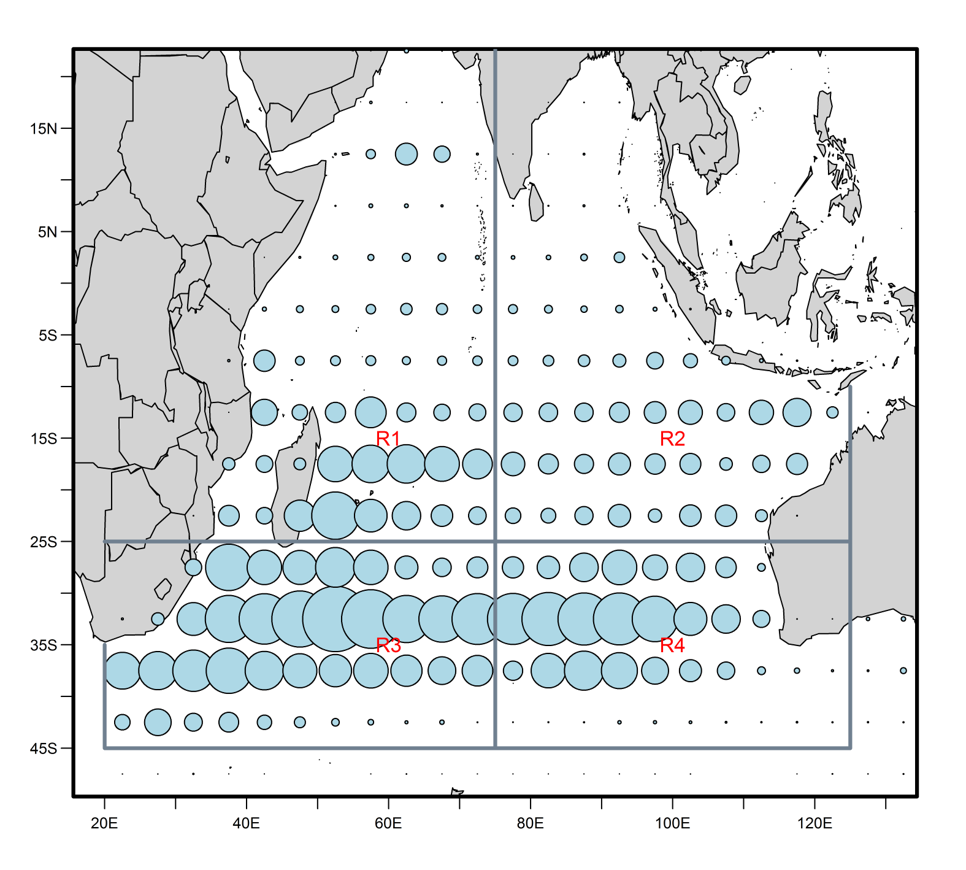
\includegraphics[width=0.75\textwidth]{figures/alb-map.png} 
\caption{Distribution of Indian Ocean albacore tuna catches by assessment areas.}
\label{fig:map}
\end{figure}

\begin{figure}
        \centering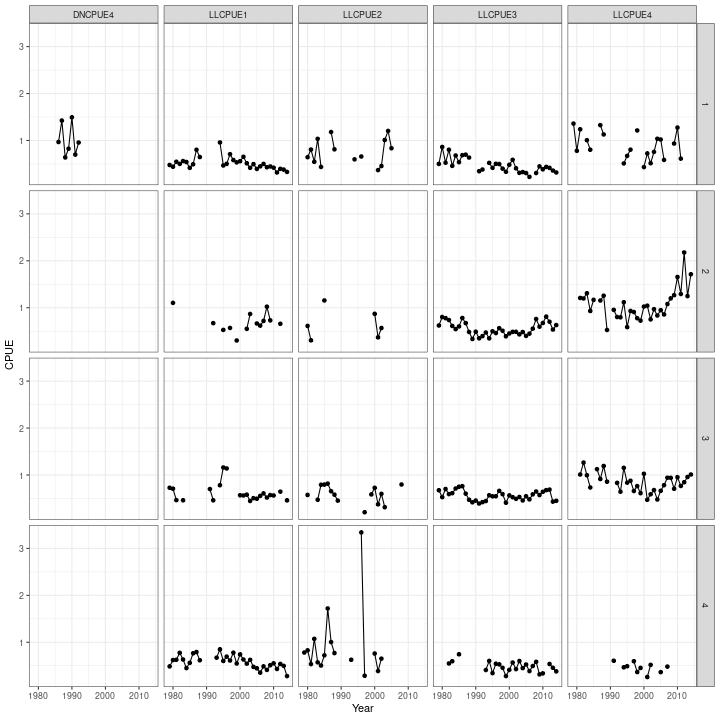
\includegraphics[width=0.75\textwidth]{figures/cpue.png}
        \caption{Indices of relative abundance for longline catch per unit effort by region and season.}
        \label{fig:u}
\end{figure}

\begin{figure}[ht!]\centering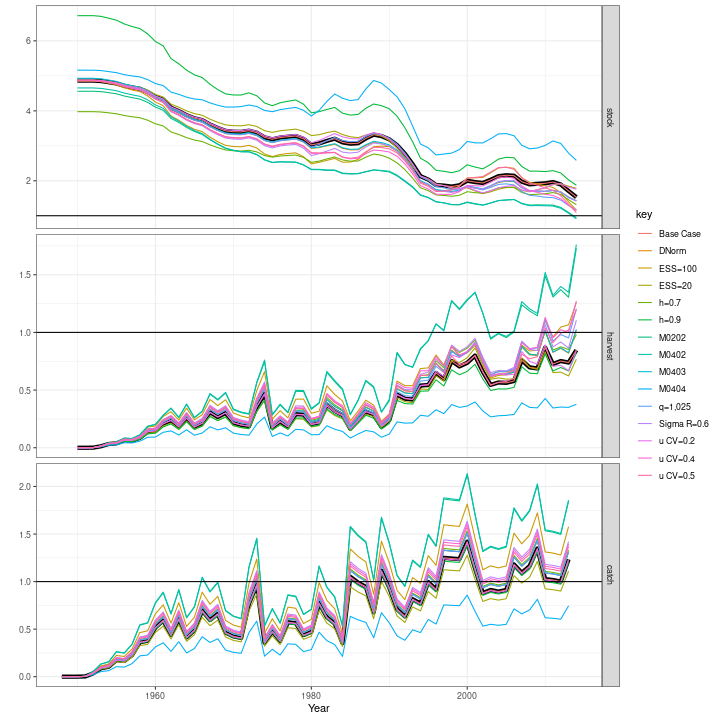
\includegraphics[width=0.75\textwidth]{figures/main-trends-1.png} \caption{Time series of spawning stock biomass and fishing mortality relative to $MSY$ target reference points for the main effects of the Indian Ocean albacore tuna assessment model grid.}
\label{fig:ts}
\end{figure}

\begin{figure}[ht!]\centering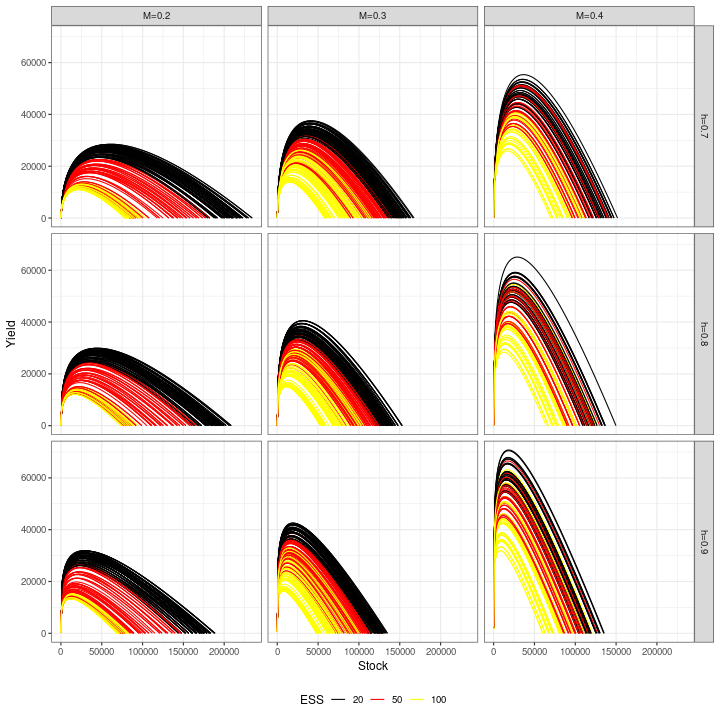
\includegraphics[width=0.75\textwidth]{figures/pf-grid-1.png} 
\caption{Production by steepness and mature natural mortality}
\label{fig:pf}       
\end{figure}

\begin{figure}
     \begin{subfigure}[b]{0.5\textwidth}
               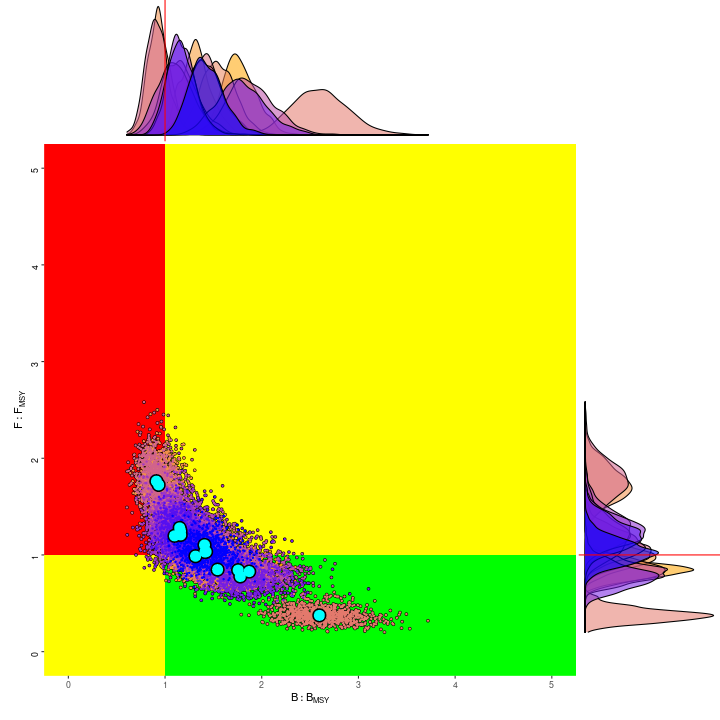
\includegraphics[width=\linewidth]{figures/kobe-main-1.png}
                \caption{Main effects with estimation error.}
                \label{fig:kobe-main}
     \end{subfigure}%
       \begin{subfigure}[b]{0.5\textwidth}
                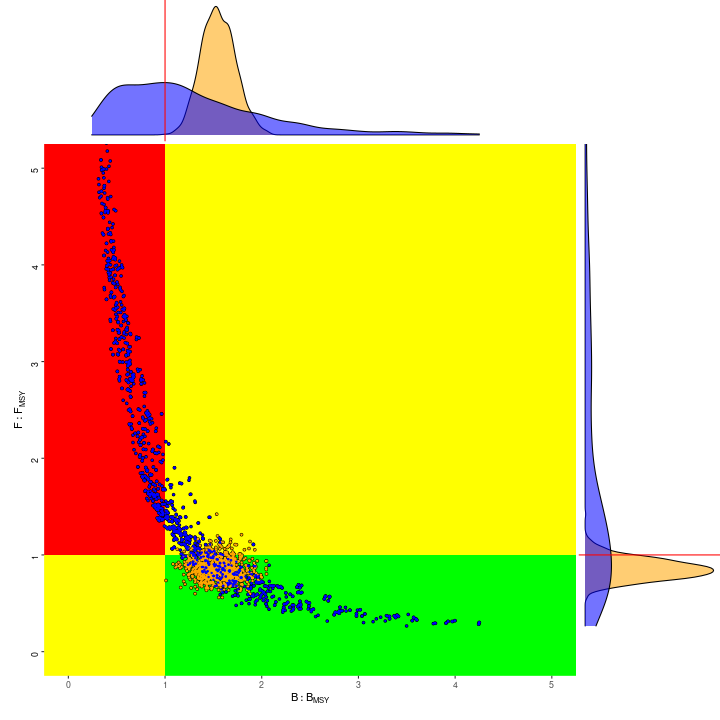
\includegraphics[width=\linewidth]{figures/kobe-bg-1.png}
                \caption{Reference case and grid with model.}
                \label{fig:kobe-bg}
     \end{subfigure}%
    \caption{Kobe phase plots showing spawning biomass ($B$) and fishing mortality ($F$) relative to $MSY$ target reference points. Within model uncertainty was approximating using multivariate log-normal distribution derived from Hessian matrix (MVLN) with cyan points denoting the median}\label{fig:kobe}
\end{figure}

%\begin{figure}[ht!]\centering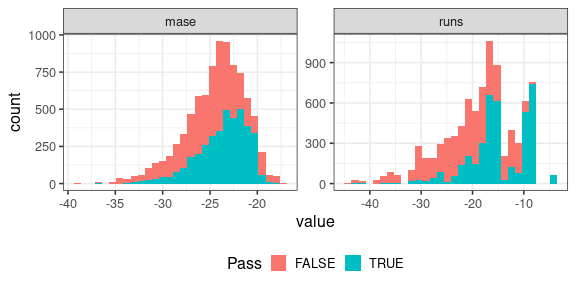
\includegraphics[width=0.75\textwidth]{figures/cf-1.png} \caption{Summary of weighting diagnostics.}\label{fig:wts} \end{figure}

%\begin{figure}[ht!]\centering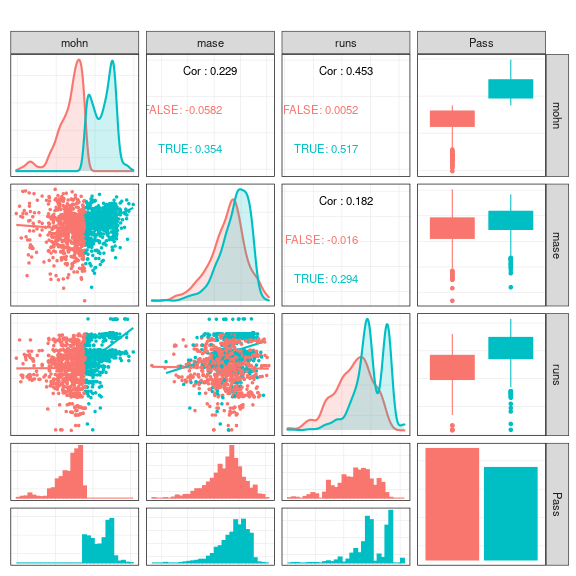
\includegraphics[width=0.75\textwidth]{figures/ggpair-1.png} \caption{Correlations between weighting diagnostics.}
%\label{fig:wts}       
%\end{figure}


\begin{figure}
        \begin{subfigure}[b]{0.5\textwidth}
           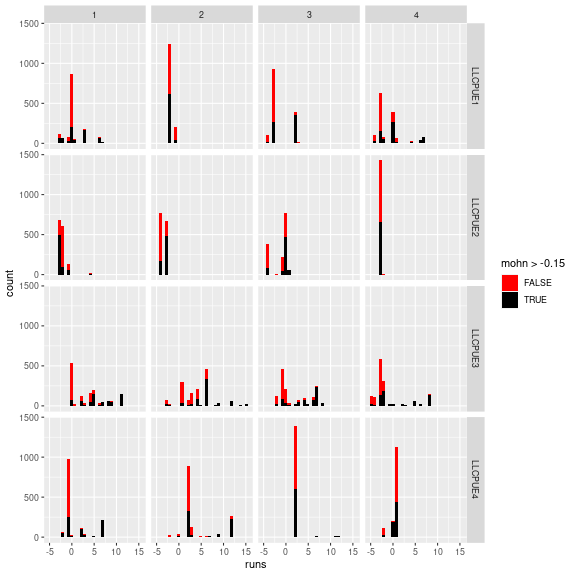
\includegraphics[width=\linewidth]{figures/runs.length-1.png}
                \caption{Runs test length of longest run - maximum run}
                \label{fig:runs}
                \end{subfigure}%
                \begin{subfigure}[b]{0.5\textwidth} 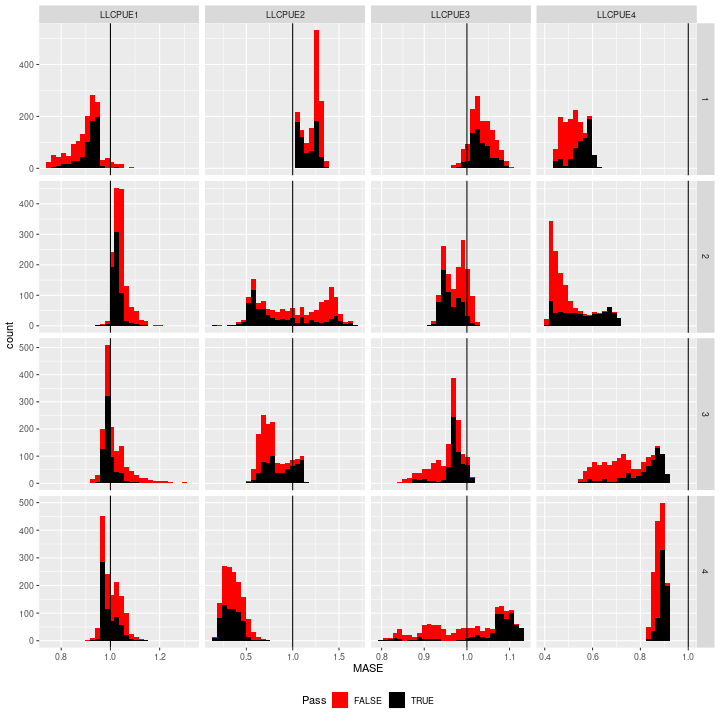
\includegraphics[width=\linewidth]{figures/mase-1.png}
                \caption{MASE}
                \label{fig:mase}
        \end{subfigure}%
        \caption{Summary of runs test and MASE.}\label{fig:mase}
\end{figure}

\begin{figure}[ht!]\centering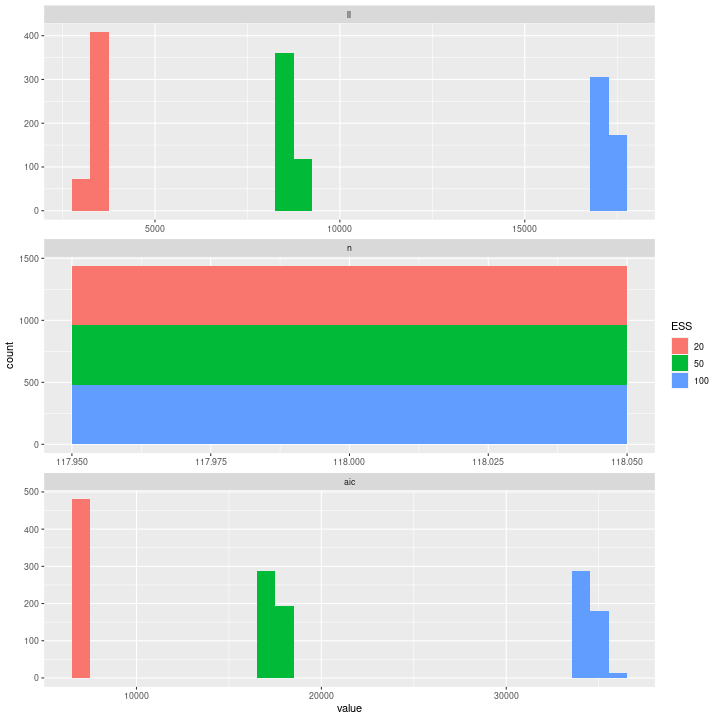
\includegraphics[width=0.75\textwidth]{figures/aic-1.png} \caption{Loglikelihood and AIC}\label{fig:aic} \end{figure}


\clearpage
\newpage
\begin{figure}[ht!]\centering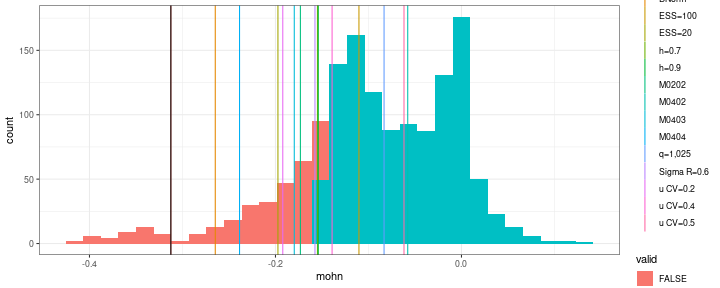
\includegraphics[width=0.75\textwidth]{figures/mohn-hist-1-1.png}  \caption{Summary of Mohn's 1-step $\rho$ for the for the 1440 assessment models in the Indian Ocean albacore tuna grid, with main effects indicated by the vertical lines.} 
\label{fig:mohn-1}       
\end{figure}

\begin{figure}[ht!]\centering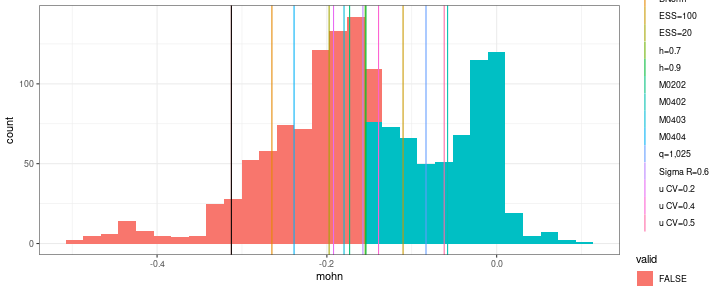
\includegraphics[width=0.75\textwidth]{figures/mohn-hist-1.png}  \caption{Summary of Mohn's $\rho$ 3-step for the 1440 assessment models in the Indian Ocean albacore tuna grid, with main effects indicated by the vertical lines.} 
\label{fig:mohn}       
\end{figure}

\clearpage
\newpage
\begin{figure}[ht!]\centering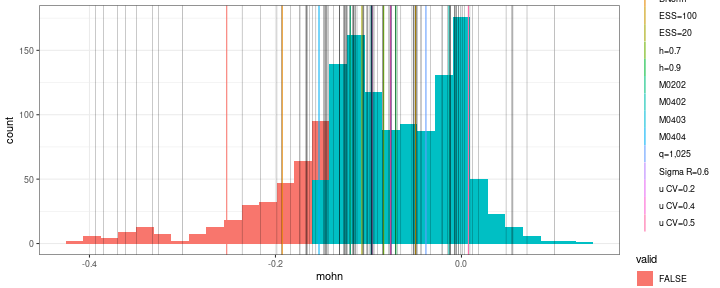
\includegraphics[width=0.75\textwidth]{figures/mohn3-hist-corner-1.png}  \caption{Summary of Mohn's 1-step $\rho$ for the for the 1440 assessment models in the Indian Ocean albacore tuna grid, with corners indicated by the vertical lines.} 
\label{fig:mohn-1-corner}       
\end{figure}

\begin{figure}[ht!]\centering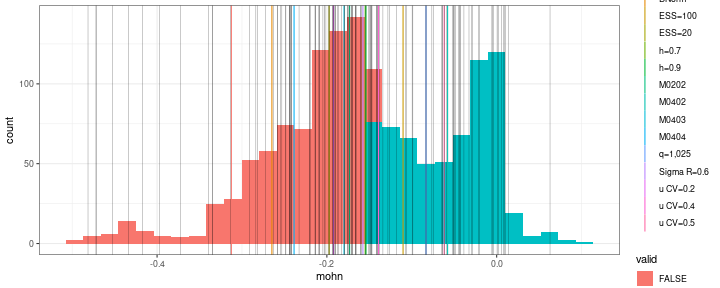
\includegraphics[width=0.75\textwidth]{figures/mohn-hist-corner-1.png}  \caption{Summary of Mohn's $\rho$ 3-step for the 1440 assessment models in the Indian Ocean albacore tuna grid, with corners indicated by the vertical lines.} 
\label{fig:mohn-corner}       
\end{figure}

\newpage
\begin{figure}[!ht]
	\centering
	\begin{subfigure}{0.9\textwidth}
		\centering
		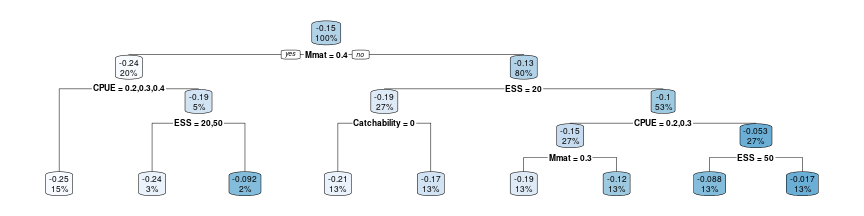
\includegraphics[width=\textwidth]{figures/a-tree-1.png}
		\caption{Regression Tree}
		\label{fig:tree}
	\end{subfigure}
	\hfill
	\begin{subfigure}{0.9\textwidth}  
		\centering 
		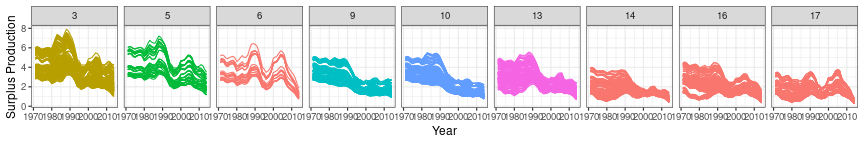
\includegraphics[width=\textwidth]{figures/a-tree-biomass-1.png}
		\caption{SSB}
		\label{fig:tree-b}
	\end{subfigure}
	\begin{subfigure}{0.9\textwidth}  
		\centering 
		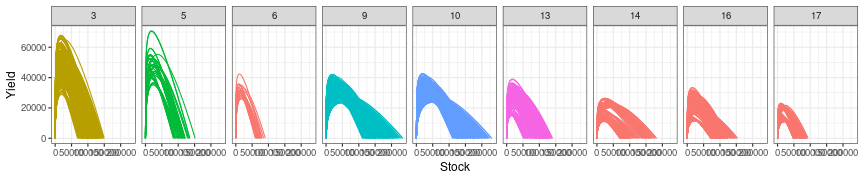
\includegraphics[width=\textwidth]{figures/a-tree-pf-1.png}
		\caption{Production Function}
		\label{fig:tree-pf}
	\end{subfigure}
	\begin{subfigure}{0.9\textwidth}
		\centering
	    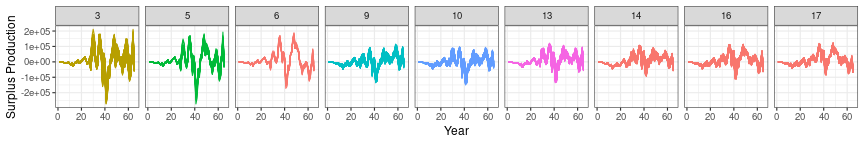
\includegraphics[width=\textwidth]{figures/a-tree-sp-1.png}
		\caption{Surplus Production}
		\label{fig:tree-sp}
	\end{subfigure}
	\caption{Mohn's $\rho$ classification tree with emergent properties.}
	\label{fig:tree}
\end{figure}


%\begin{figure}[ht!]\centering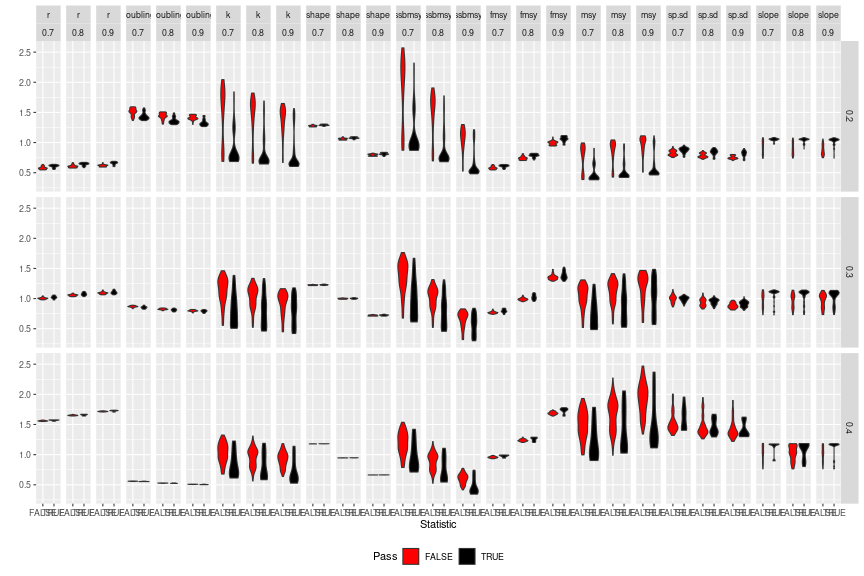
\includegraphics[width=1\textwidth]{figures/param-box-mohn3-1.png}\caption{Summary statistics, will re-do for $F/F_{MSY}$, $B/B_{MSY}$, $r$, $K$, $p$ and $sd(sp)$, and population doubling time.}\label{fig:smry}\end{figure}

\begin{figure}[ht!]\centering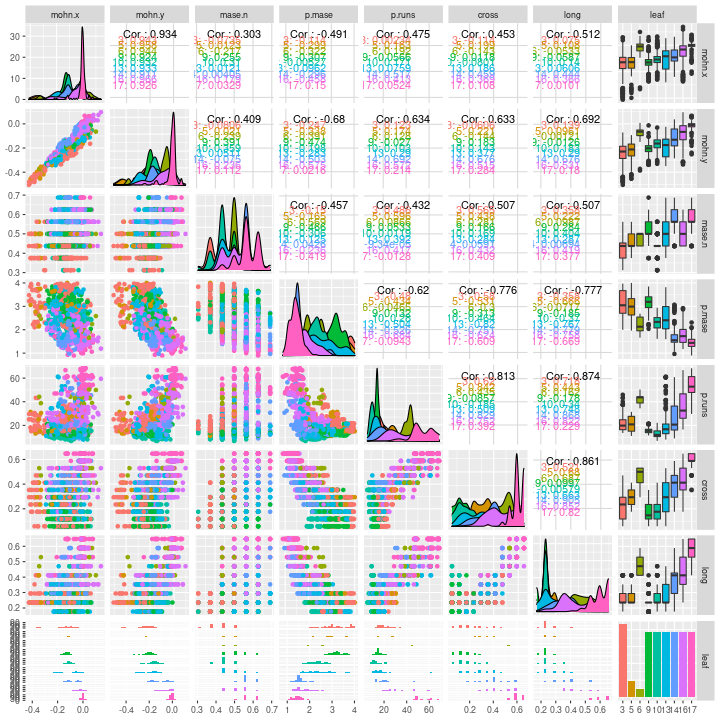
\includegraphics[width=0.75\textwidth]{figures/cluster.tree.2-1.png} \caption{Comparison of Mohn's $\rho$ and $-2log(p)$ for runs test and Diabold Marino test, ...}\label{fig:xxx} \end{figure}

\begin{figure}
        \begin{subfigure}[b]{0.5\textwidth}
                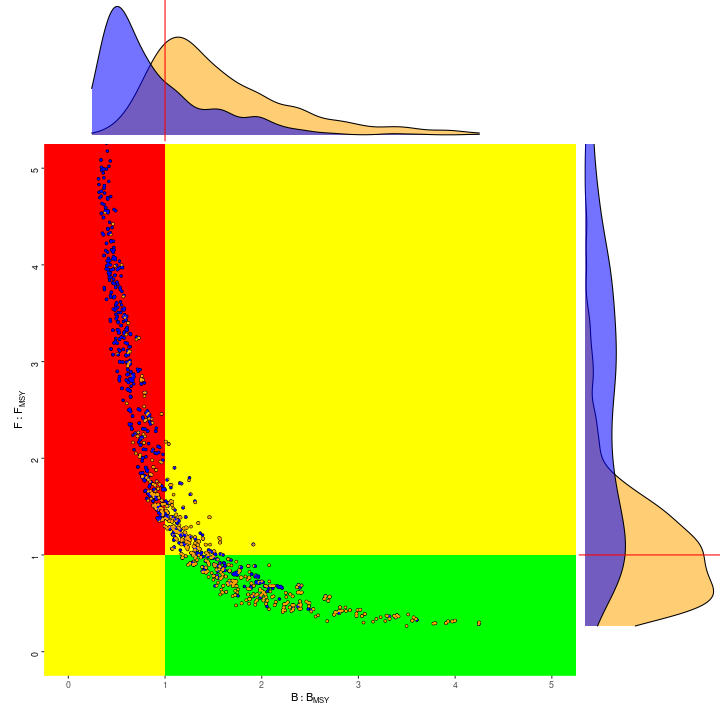
\includegraphics[width=\linewidth]{figures/kobe-mohn3-1.png}
                \caption{Kobe}
                \label{fig:kobe-wt}
        \end{subfigure}%
        \begin{subfigure}[b]{0.5\textwidth}
                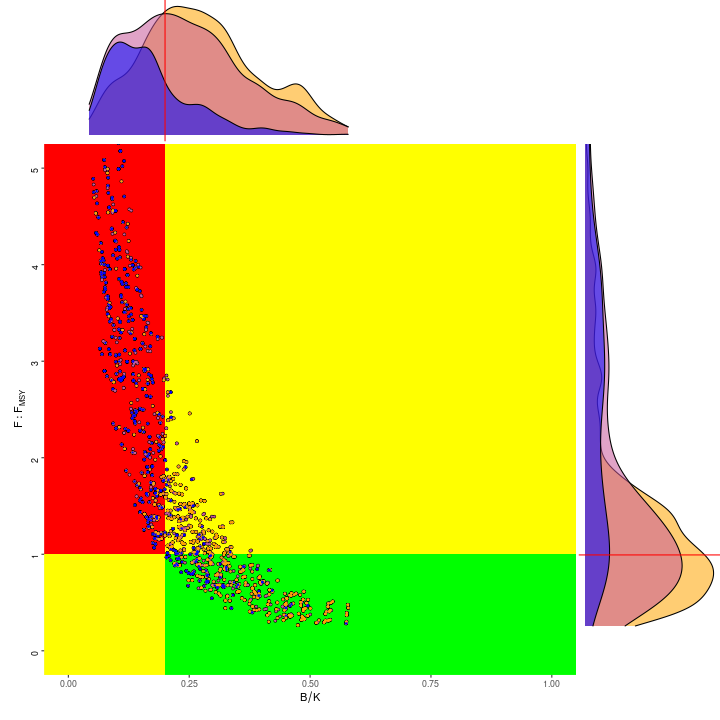
\includegraphics[width=\linewidth]{figures/majuro-mohn3-all-1.png}
                \caption{Majuro}
                \label{fig:majuro-wt}
        \end{subfigure}%
        \caption{Phase plots for all 1440 grid models, with equal, AIC, and skill weighting identifying models that pass the Mohn's $\rho$ test for hindcasts with 3 year ahead forecasts .}
        \label{fig:phase-wt}
\end{figure}

\end{document}

 $w_M = \frac{exp(-(1/2)\text{AIC}_M)}{\sum_{M\in S}{exp(-(1/2)\text{AIC}_M)}}$
\section*{Introduction}


The adoption of the Precautionary Approach to fisheries management \citep[PA,][]{garcia1996precautionary} requires a formal consideration of uncertainty. This had led to the use of Management Strategy Evaluation (MSE) is to develop robust advice that can still meet management objectives despite uncertainty. When conducting MSE Operating Models (OMs) are used to represent alternative hypotheses about the dynamics of the system. The most common procedure when is to fit to the available data on the basis of some statistical criterion, such as a Maximum Likelihood. The aim of this conditioning process is to reject OMs that do not fit the data satisfactorily, and are inconsistent with the actual dynamics.  

 There has been a trend when conducting MSE to use integrated assessment models for conditioning, as this allows different sources of data to be combined into a single model by a joint likelihood  \citep[e.g.][]{doubleday1976least,fournier1982general,maunder2013review}, as this allows scientists seek to use the models to capture all knowledge about stock size and productivity \citep{hilborn2003state}. Problems remain, however, including a lack of information on spatial and temporal processes that may affect stationarity,  density dependence, and conflicts between datasets. Misspecification of key parameters or assumptions in integrated stock assessment models can strongly impact the estimates of quantities of management interest, such as stock depletion and biomass at maximum sustainable yield \citep{mangel2013perspective}. Therefore, the impact of uncertainty about resource dynamics is commonly evaluated by the use of a grid-based design that considering alternative model structure, datasets and parameters \citep{sharma2020mse}. 
 
 Integrated models are commonly used to conditioning Operating Models (OMs) as part of Management Strategy Evaluation (MSE). This involves fitting an OM of the resource dynamics to the available data on the basis of some statistical criterion, such as a Maximum Likelihood.  The aim of conditioning is to reject OMs that do not fit the data satisfactorily, and are consequently inconsistent with the actual situation observed and therefore implausible. Therefore, when conditioning OMs the intention is not to find a "best assessment" but a limited set of OMs with high plausibility, which include the most important uncertainties in the model structure, parameters, and data. Plausibility may be estimated formally based on some statistical approach, or specified based on expert judgement, and can be used to weight performance statistics when integrating over results for different scenarios (OMs). The methods developed in the cookbook can be used to do this. 
 
 To date, however, little effort has gone into weighting of the different models, e.g. based on ensemble modelling. Advice, however, depends on the weights given to the different models when post processing, and critically the original choice of models. Therefore questions that need to be answered in the conditioning are does the model presents a good fit to the data and is it able to predict the response to fishing \citep{carvalho2020cookbook}. We therefore develop a schema for weighting and potential rejection of stock assessment model scenarios, and compare different metrics to simple skill-based weighting (SW).
 

\section*{Material and Methods}

An Operating Model for the albacore tuna (\textit{Thunnus alalunga}) fishery and stock in the Indian Ocean has been developed by the Indian Ocean Tuna Commission (IOTC) to evaluate the performance of alternative Management Procedures (MPs).  The Operating Model (OM) was conditioned using stock synthesis \citep[SS3][]{MethotW2013} based on current best knowledge and data \citep{ptmt2014}. Datasets include records of catches and landings, indices of abundance based on catch per unit (CPUE), and  length and ages compositions from samples. Reformulating model structure, however, is time consuming and so scenarios were based on the choice of parameters for which there is insufficient information in the data to estimate and data weighting. 

\subsection*{Material}

The assesssment partitions the Indian Ocean into four regions, divided latitudinally along the 25$^{\circ}$S parallel and longitudinally along the 75$^{\circ}$E meridian. Aggregated catches (in numbers of fish) for the Japanese and Taiwanese LL fleets, for the 1950-2014 period, are shown. From \citep{LangleyH2016}, figure \ref{fig:map} show the distribution of catches across the areas defined in the assessment. The model includes a total of 11 fisheries, including in this case an aggregaqted Longline fishery for each of the four regions. For a detailed explanation of the data and fleets included in each of these fisheries, please refer to \citep{LangleyH2016}. A new set of standardized CPUE indices has been derived using generalized linear models (GLM) operational from longline catch and effort data provided by Japan, Korea and Taiwan, China. \citep{HoyleKL2016}. The operating model conditioning used the same series as the final runs of the stock assessment \citep{LangleyH2016}, a combined industrial longline series, on each of the four areas, and restricted to the 1979-2014 period (Figure \ref{fig:cpues}). Of these four areas, area 3 is considered to represent the core of the distribution of the stock. The management procedures tested make use of a single CPUE, taken to be that corresponding to area 3.

The distribution of catches by assessment areas are shown in are shown in figure \ref{fig:map}.
   
Fisheries data is in general less informative that would be ideal when it comes to estimating a large number of model parameters, which are often correlated. In the case of the Indian Ocean albacore stock, a number of reasons are limiting our ability to obtain reliable model fits. Problems exists with the data completeness and quality \citep{IOTC2016WPTmT0607}, not limited to but including total catch statistics, length distribution in catches, and biological information. We also depend on our ability to produce sensible indices of changes in abundance in the stock based only on Catch-per-unit-effort data from commercial fleets, where issues of targeting, operating and others are all known to influence the relationship between stock abundance and CPUE, despite recent work on standardization of the longline CPUE series for this stock \citep{oyleKL2016}.

The seven factors currently considered in the structural uncertainty grid for the albacore OM are shown in  table \ref{tab:om})

A common unknown in most stock assessment models, the base case considered in the stock assessment session was supplemented with alternative values of higher and lower M for either all ages, or different for juveniles (ages 0 to 4) and adults (age 5 or older), for a total of five possibilities. Two values were considered for the true variability of recruitment in the population, 0.4 and 0.6. Three values for the steepness (h) of the stock-recruitment relationship are being used: 0.7, 0.8, and 0.9. The Beverton and Holt stock-recruit model implemented. Four values for the coefficient of variation in the CPUE series were included: 0.2, 0.3, 0.4 and 0.5. Three values were used for the relative weight of length sampling data in the total likelihood, through changes in the effective sampling size parameter, of 20, 50 and 100. This alters the relative weighting of length samples and CPUE series in informing the model about stock dynamics and the effects of fishing at length. Two scenarios were considered for the effective catchability of the CPUE fleet. On the first one it was assumed that the fleet had not improved its ability to fish for albacore over time, or that any increase had been captured by the CPUE standardization process. An alternative scenario considered a 2.5\% increase in catchability by correcting the CPUE index to reflect this.  Two possible functional forms for the selectivity of the CPUE LL fleet were considered: a logistic function (Log), where selectivity stays at the maximum level, or double normal (DoNorm), where selectivity drops at some point in the age range.


\subsection*{Methods}

The performance of multimodel ensembles depends on the weights given to the different models in postprocessing. Although still common practice, equal weighting of all models in a grid or ensemble may result in biased advice if too much weight is assigned to models that fit the data poorly or have low have poor prediction skill \citep{kell2020yft}.

We therefore explore a number of different potential weighting schema, and methods for selecting and rejecting OM scenarios, and compare equal weighting (EW), with simple skill-based weighting (SW) \citep{casanova2009weighting}.

\subsubsection*{Weighting}

%Considering alternative structures and datasets means that it difficult to select models using metrics such as AIC. Therefore retrospective analysis is commonly used to evaluate the stability of stock assessment estimates of model estimates such as stock biomass and exploitation level. Stability is measured using Mohn's $\rho$ a measure of bias. Shrinking estimates of stock status in the last year to the recent mean can help reduce Mohn's $\rho$. Shrinkage, in statistics, however, is used to reduce mean squared error (MSE), at the expense of bias. The use of model based quantities, however, means that bias can not be quantified, and may result in forecasts having little prediction skill. We therefore extend retrospective analyses to include prediction. 

\begin{description}
\item[Expert] Stakeholder concerns and expert opinion, assigned “a-priori”, without consideration of model fit.
 \begin{itemize}
    \item How were scenarios selected?, e.g. through an elicitation process \citep{leach2014identification}?
\end{itemize}
\item[Convergence] Model convergence criteria of the estimation algorithm. 
\begin{itemize}
    \item max gradient? This is normally achieved by jittering, however this is difficult to do in this case where 1440 grids are run. Therefore we explore what factors result in poor convergence.
\end{itemize}
\item[Diagnostics] Reliability of the model based on residual diagnostics
 \begin{itemize}
    \item Use runs tests to check for randomness in the residuals 
\end{itemize}
 \item[Fit] The fit of the model to the data
 \begin{itemize}
    \item Likelihood, we do not use AIC due to problems in weighting and the fact that since the number of parameters only changes for 1 scenario the AIC and likelihoods are equivalent. Using the likelihood also allows us to look at data components.
\end{itemize}
\item[Plausible parameters] The plausibility of the estimates of the parameters representing the dynamics
 \begin{itemize}
    \item  $r$, $K$ and $p$, i.e. production functions
\end{itemize}
\item[Plausible results] Time series dynamics and process error.
\begin{itemize}
    \item ACF of biomass
    \item clockwise SP
    \item var(SP)
\end{itemize}
\item[Stability] Retrospective
https://www.overleaf.com/project/5f06c2b7d4ece70001d5c362\begin{itemize}
    \item traditional Mohn's $\rho$
\end{itemize}
\item[Prediction Skill] Model outputs
 \begin{itemize}
    \item 3 year ahead Mohn's $\rho$ 
\end{itemize}
\item[Prediction Skill] Model free
\begin{itemize}
    \item MASE for CPUE
\end{itemize}
\end{description}

\subsubsection*{Runs Test}

Analysis of residuals is a common way to determine a model’s goodness-of-fit \citep{Cox1968general}, since  non-random patterns in the residuals may indicate model misspecification, serial correlation in sampling/observation error, or heteroscedasticity. 

When inspecting residuals, however, there is a danger of hypothesis fishing and if multiple true hypotheses are tested it is likely that some of them will be rejected. Therefore it is valuable to reserve part of the data for validation, so that a pattern’s significance is not tested on the same data set which suggested the pattern.


If the process of interest shows only random variation, the data points will be randomly distributed around the median. Random meaning that we cannot know if the next data point will fall above or below the median, but that the probability of each event is 50\%, and that the data points are independent. Independence means that the position of one data point does not influence the position of the next data point, that is, data are not auto-correlated. If the process shifts, these conditions are no longer true and patterns of non-random variation may be detected by statistical tests. Various statistics exist to evaluate residuals and nonparametric tests for randomness in a time-series include: the runs test, the sign test, the runs up and down test, the Mann-Kendall test, and Bartel’s rank test.

Non-random variation may present itself in several ways. If the process centre is shifting due to improvement or degradation we may observe unusually long runs of consecutive data points on the same side of the median or that the graph crosses the median unusually few times. The length of the longest run and the number of crossings in a random process are predictable within limits and depend on the total number of data points in the run chart \citep{anhoj2015diagnostic}.

A shift signal is present if any run of consecutive data points on the same side of the median is longer than the prediction limit, round(log2(n) + 3). Data points that fall on the median do not count, they do neither break nor contribute to the run \cite{schilling2012surprising}. A crossings signal is present if the number of times the graph crosses the median is smaller than the prediction limit, qbinom(0.05, n - 1, 0.5) \citep{chen2010impacts}. n is the number of useful data points, that is, data points that do not fall on the median. The shift and the crossings signals are based on a false positive signal rate around 5\% and have proven useful in practice.
\input{Hindcast}
\subsubsection*{Generating delta-MVLN Kobe posteriors}

Generate Kobe posteriors from a MVLN distribution requires the means and the variance-covariance matrix (VCM) of $log(SSB/SSB_{MSY})$ and $log(F/F_{MSY})$. Let $u = SSB/SSB_{MSY}$ and $v = F/F_{MSY}$  and $x = log(u)$ and $y = log(v)$ , then the $VCM$ has the form:
    			
\begin{equation}
VCM_{x,y} =
\begin{pmatrix}
\sigma^2_x & cov_{x,y}  \\
cov_{x,y} & \sigma^2_y
\end{pmatrix}
\end{equation*}

where  is the variance of x,  is the covariance of y and  is the covariance of x and y.  The quantities that can be directly extracted from Stock Synthesis are: (1) MLEs, asymptotic standard errors (SE) and correlation of $SSB/SSB_{MSY}$  and $F/F_{MSY}$. 
The construction of the  therefore requires to conduct a few normal to lognormal transformations. First, we approximate  and  as:

\begin{equation}
\sigma^2_x = \disp log\left(1+\left(\frac{SE_u}{u}\right)^2\right)  
\quad 
\end{equation}

and

\begin{equation}
\sigma^2_x = \disp log\left(1+\left(\frac{SE_v}{v}\right)^2\right)  
\quad 
\end{equation}

where  and  is the asymptotic standard error estimate for $u = SSB/SSB_{MSY}$ and $v = F/F_{MSY}$. Second, the covariance of x and y can then be approximated on log-scale by:

\begin{equation}
COV_{x,y} = \disp log \right{1+ \rho_{u,v} \sqrt{\sigma^2_x\sigma^2_y}\right \quad 
\end{equation}

where  donates the correlation of u and v.
To generate the desired KPD for $SSB/SSB_{MSY}$  and $F/F_{MSY}$, we use a multivariate random generator, available in the R package ‘mvtnorm’, to obtain a large number (nsim = 10,000) of x and y pairs, such that

\begin{equation}
kobe_{x,y} = \disp MVN{\mu_{x,y},VCM_{x,y}) 
\quad 
\end{equation}

where  is the vector of the MLEs x and y. The joint MVLN distribution of $-SSB/SSB_{MSY}$  and $-F/F_{MSY}$ is then obtained as the exponential of $kone_{x,y}$.



There are a variety of frequentist model-weighting strategies ranging from giving all models in S a weight related to the AIC (Akaike information criterion) or BIC (Bayesian information criterion) of each model, to an interpolation between two extreme cases. We present an AIC-based weighting strategy called smooth AIC weights that was first presented by Buckland et al. (1997). In smooth AIC weighting, the weights are given by:  
wM=exp(−(1/2)AICM)∑M′∈Sexp(−(1/2)AICM′).
(6)

It is suggested to subtract the minimum AIC from each model AIC to avoid numerical issues when taking exponents.

%In age-structured models, there is an implicit production function, and changes in productivity can occur due to process error modelled as variability in recruitment and selection pattern. In the biomass-dynamic models with an explicit production function, process error is modelled explicitly.

In age-structured models, density dependence is mainly accounted for by the stock-recruitment relationship. Cury et al. (2014), however, showed that in most cases the stock-recruitment relationship used to estimate productivity and determine reference points, has poor estimation/predictive power and the environment has a larger effect on productivity, a result confirmed by other studies (e.g. Szuwalski et al., 2015, 2019; Free et al., 2019), and observed 100 years ago by Hjort (1914). Whereas in ICCAT assessments growth, maturation and natural mortality are assumed not to have varied despite the significant changes in the environment and stock biomass seen.

Hilborn (2001) therefore recommended looking at patterns of change in surplus production (SP) since these may contain evidence of changes in the growth and mortality components of production, which are typically not represented in models currently used for stock assessment and management. 

Walters et al. (2008) argued that plotting of surplus production (SP) against biomass (B) should be one of the basic pieces of information presented in all stock assessments since the plots provide a check on whether there has been non-stationarity in the annual surplus production, i.e. whether similar B levels have exhibited similar SP at different historical times. This is important for management as it checks whether predictions of changes in biomass (Bt+1−Bt) can be made reliably based on catch and Bt. Plots of SP v B therefore provide a summary of stock performance and include effects not necessarily included in stock assessment models.

The effects not included in the production function used to predict SP can be modelled by a process error term # t.

				$B_{t+1} = B_t − C_t + SP_t + ε_t$

Process error on biomass can account for model structural uncertainty as well as natural variability of stock biomass due to stochasticity in recruitment, natural mortality, 4growth, and maturation (Francis and Hilborn, 2011; Meyer and Millar, 1999; Thorson et al., 2015).

We, therefore, examine the relationships between surplus production and biomass . To do this, we estimate annual surplus production as the change in stock size plus catch (i.e. $B_t – B_{t+1} + C_t$). We then plot the resulting time series of S and B to identify patterns of variation in S. The process error was then sampled from SS3 stock trajectories as the difference between the deterministic expectation of biomass and its stochastic realisation, such that:

				$ε_t = SB_{t+1} - (SB_t + SP_t − C_t)$ 



\newpage
\section*{Results}

\begin{itemize}
   \item Time series of catch, and spawning stock biomass and fishing mortality relative to $MSY$ target reference points are shown in figure \ref{fig:ts} for the base case (black line) the main effects. Catches have increased since the 1950s, and in the last two decades have varied just above $MSY$. This has resulted in an increase in $F$ and a decrease in $SSB$, although the stock is assessed to be above $SSB/B{MSY}$ and in only a few cases is $F$ above $F_{MSY}$.  

   \item The production functions from which the $MSY$ reference points are derived are shown in figure \ref{fig:pf}. There are two main features a change in the shape of the production function with steepness, and an increase in scale as the natural mortality of adults increases or the length composition effective sample size decreases. The increase in adult M, the shape of the production function, results in the stock becoming more robust to exploitation, since to explain the catches the stock most be more productive, as seen by the increase of the slope at the origin, and hence population growth rate ($r$)  

   \item Kobe phase plots (figure \ref{fig:kobe}) showing $SSB/B_{MSY}$ and $F/F_MSY$ in the terminal year are shown for the main effects with estimation error approximated using a multivariate log-normal, (cyan points denote the median) in figure \ref{fig:kobe-main}, and the base case is compared to the full grid in figure \ref{fig:kobe-bg}. The base case only gives a X\% chance of being in the green quadrant ($SSB \gt SSB_{MSY}$ and $F \le F_{MSY}$) when estimation error is considered. Although only 1 main effects (M0202?) is in the red quadrant, X\% are in the red quadrant when estimation error is considered, while when model error is considered this increases to Y\%. 
   
   \item Summary of Mohn's $\rho$ for the for the 1440 assessment models in the Indian Ocean albacore tuna grid, with main effects indicated by the vertical lines (Figure \ref{fig:mohn}). Four of the main effects fail the Mohn's $\rho$ test. There appears to be bi-modality with one mode centred on 0, i.e. some scenarios perform very well compared to the main effect and base case.
   
   \item This shows that uncertainty is underestimated if only estimation error is considered. This implies over-fitting and a subsequent reduction in variance at the expense of bias. Figure \ref{fig:runs} therefore compares the runs tests based on the model residuals to the prediction residuals for the entire grid. The number of crossings (figure \ref{fig:runs-cross}) and the length of the longest run (figure \ref{fig:runs-long} and the MASE (figure \ref{fig:mase}). Most of the scenarios and indices pass the crossings test, while performance for the length of the longest run is poorer. Indices 2 and 3 perform best. The value of Mohn's $\rho$ does not appear to have an impact. 
   
   \item The results for MASE from the model-free hindcast are different from the runs tests, in that Mohn's $\rho$ does appera to have an effect, i.e. a scenario and index has a value of $MASE \gt 1$ it also tends to have lower prediction skill.  While the relative performance of indices 2 and 3 is similar to the runs tests, index 4 now has good performance.
   
   \item The p-values by scenarios for MASE and the runs test are compared to Mohn's $\rho$ in figure \ref{fig:wts}. These show that in the sceanrios with good prediction skill indices perform better, based on MASE. The runs test does not appear to be an indicator of prediction skill, potentially due to overfitting. 

   \item A Regression tree identifying factors that influence Mohn's $\rho$ for the 1440 assessment models is shown in Figure \ref{fig:tree}. This also shows the time series of SSB (\ref{fig:tree-b}), production functions (\ref{fig:tree-pf}), and time series of surplus production (\ref{fig:tree-sp}). The first split is on natural mortality of the adults, if this is equal to 0.4 then the Mohn's $\rho$ test is failed, otherwise it is passed. These, as seen above have lower estimated values of $B_{MSY}$ and $MSY$. The two exceptions are for M=0.3 and CPUE = 0.2 \& 0.3 when it fails, and M=0.4 and CPUE=0.5 \& ESS = 100 when it passes. In other word the biggest impact on prediction skill is M, since high M results in a large productive stock which is not supported by the hindcast. High M is only plausible if you ignore the CPUE and fit to the length data. 
   
  \item Weighted phase plots are presented in figure \ref{fig:phase-wt} for equal, simple skill based, and AIC weighting. These are for targets (Kobe \ref{fig:kobe-wt}) and limits (Majuro \ref{fig:majuro-wt}). 

  \item Figure \ref{ref:grid} summarises a variety of summary metrics by adult M and steepness for Mohn's $\rho$. $SSB/B_{MSY}$ (\ref{fig:grid-bmsy}), $B_{lim}$ (\ref{fig:grid-blim}), $F/F_{MSY}$ (\ref{fig:grid-fmsy}), $r$ (\ref{fig:grid-r}), $K$, (\ref{fig:grid-k}), $p$, (\ref{fig:grid-p}), $sd(sp)$, (\ref{fig:grid-sp}), and Population doubling time (\ref{fig:grid-dt}). There is some modality due to catchability, particulary in current biomass status and $K$.  Again the biggest impact is adult M. 

\end{itemize}




\clearpage
\newpage
\newpage
\section*{Discussion}


When developing metrics as in any indicator, the total number should be minimised, complementary and non-redundant (Shin et al. 2010; Kershner et al. 2011). They should also be robust proxies for relevant attributes, and need to be screened using appropriate selection criteria \cite{kell2020roc}. To be effective a metric should be robust, so that it still functions despite uncertainty \parencite{radatz1990ieee, zhou1996robust}. To be robust an metric should be both reliable and stable. A metric has high reliability if despite uncertainty it provides an accurate result, and it is stable if despite random error, similar results are produced across multiple trials. 

\begin{itemize}
    \item The aim of this work was to evaluate the use of full factorial designs for representing uncertainty in stock assessment. In particular to identify the assumptions that impact the perception of stock dynamics and status, and develop tools for weighting or rejecting stock assessment scenarios.
  
    %\item The Indian Ocean Albacore MSE used Stock Synthesis to develop scenarios based on parameters that are difficult to estimate (i.e. M, steepness, and selectivity) and the relative weightings of the indices of abundance and the length data. The choice of OMs is important as the \textit{best} Management Procedure is determined by the choice of hypotheses represented by the OM. It seldom possible, however, to assign plausibility to the different scenarios, therefore the rationale for the grid design is of fundamental importance.

    %\item Need to consider the future not just the past
    
    \item The absence of retrospective patterns in model quantities such as stock biomass, is not sufficient to validate models based on model outputs, since a small RE could be achieved by a model that used no data.  Therefore conduct a hindcast.
    
    \item Can only validate models on observations and not model outputs, therefore need to conduct model free hindcasts to estimate prediction skill by comparing observations and to their model estimates, to explore bias, variability and prediction skill.
    
    \item Use the hindcast procedure to weight multi-model ensembles using simple skill-based weighting. A prediction skill score can be used to assign more weight on the better performing models as this has been found to improve forecasts \citep[e.g.][]{casanova2009weighting}. This can be done to weight estimates of current status relative to reference points, or weight operating models when conducting MSE. %Testing the approach on an actual case study first was informative as it provides the insight necessary to set up a study on synthetic data.

    %\item next step is assess prediction skill using model free hindcasting, as it allows comparisons to be made across model structures and datasets. Validation examines if a model family should be modified or extended and is complementary to model selection and hypothesis testing. In comparison model selection searches for the most suitable model within a family, whilst hypothesis testing examines if the model structure can be reduced. This is important as it allows alternative model frameworks to be compared and valiadated in a working group setting.

    %\item When conducting Management Strategy Evaluation (MSE) Operating Models (OMs) are commonly \citep{Sharma} conditioned using stock assessment models and a grid design to model structural uncertainty and data conflicts. However, there are two main characteristics of the stock dynamics i.e. the expected dynamics as represented by a production function and the nature of the times series. Therefore you could just run a limited number of scenarios that represent the different production functions an time series dynamics.

    \item \cite{fischer2020linking} showed that to develop robust management strategies the nature of the time series of the stock has to be considered. The importance of this is that trends and fluctuations in populations are determined by complex interactions between extrinsic forcing and intrinsic dynamics. For example, stochastic recruitment can induce low-frequency variability, i.e. ‘cohort resonance’, which can induce apparent trends in abundance and may be common in age-structured populations \citep[e.g.][]{bjoernstad2004trends, botsford2014cohort}. Such low-frequency fluctuations can mimic or cloak critical variation in abundance linked to environmental change, over-exploitation or other types of anthropogenic forcing. In feedback management systems the nature of the time series dynamics is likely to be more important than the equilibrium dynamics. 
    
    \item The objective of MSE is to develop a robust MP, so weighting of OM grids based on stock assessments is a waste of time. Since trends and fluctuations in populations are determined by complex interactions between extrinsic forcing and intrinsic dynamics. For example, stochastic recruitment can induce low-frequency variability, i.e. ‘cohort resonance’, which can induce apparent trends in abundance and may be common in age-structured populations \citep[e.g.][]{bjoernstad2004trends, botsford2014cohort}. Such low-frequency fluctuations can potentially mimic or cloak critical variation in abundance linked to environmental change, over-exploitation or other types of anthropogenic forcing. In feedback management systems the nature of the time series dynamics is likely to be more important than the equilibrium dynamics.

   \item Weighting give very different results wrt targets and limits, this is important, e.g. for MSC. Rather than arguing about the best weighting scheme better to develop robust MPs, that need to be tested for a range of plausible dynamics. 
   
\end{itemize} 



\section{Conclusions}

I totally agree on the automation, to ensure objectively and transparency. Its like MSE where you have to agree the OMs and the MP selection criteria in advance.

Also like MSE, I think we need a limited number of complementary but non-redundant metrics. For example are the runs tests,  RMSE and Mohn's rho telling us the same thing? So we are give a single attribute extra weight? Imagine you have a model with a biased index, i.e. a data conflict, that fails the runs and RMSE tests. When you do retrospective you are removing biased points so you will get a large absolute value for Mohn's rho. In contrast MASE for a model free quantity will hopefully be telling you something else. It would be best to recognise that data conflict at the start.

For this reason I  agree with Mark that ideally a model should pass all diagnostics but recognise that this isn't always possible. For example if a model fails to converge that could indicate data conflicts and model misspecification, that will bite you later if not fixed. For example when you start removing points example in the retrospective analysis and hindcasts.

Also while the delta-MVLN approach is useful, I would also like to use estimation error to check bias, i.e. by looking at prediction residuals.

\begin{itemize}
    \item In the stock assessment process hypotheses about states of nature are represented by alternative model structures and fixed parameters. Even with a design of 1440, as in this example, the choice of scenarios is arbitrary and the posterior distributions are often multi-modal.
    
    \item Considering alternative structures and datasets means that it difficult to select models using metrics such as AIC. Therefore retrospective analysis is commonly used to evaluate the stability of stock assessment estimates.  The use of model based quantities, however, means that bias can not be quantified, and may result in future predictions being being poor. We therefore extended retrospective analyses to include predictions. 
   
    \item The use of metrics based on prediction skill allows different data components and model to be compared in order to explore data conflicts and potential model misspecification. The accuracy and precision of predictions depend on the validity of the model, the information in the data, and how far ahead predictions are required. 
   
    \item Retrospective analysis is commonly used to evaluate the stability of stock assessment estimates of model estimates such as stock biomass and exploitation level. Stability is measured using Mohn's $\rho$ a measure of bias. 
    
    \item Shrinking estimates of stock status in the last year to the recent mean can help reduce Mohn's $\rho$. Shrinkage, in statistics, however, is used to reduce mean squared error (MSE), at the expense of bias. 
    
    \item The use of model based quantities, however, means that bias can not be quantified, and may result in future predictions being being poor. We therefore extend retrospective analyses to include prediction. 

    \item When developing the design for ensembles or OMs first it is necessary to choose a base case, the main effects and interactions. A problem is that hypotheses are likely to be confounded e.g. i) is High M and low steepness realistic? ii) relative weighting of ESS and CPUE CV; and iii) dome shaped selection or senescence. If we had used the approach proposed would our conclusions have differed? Use of feedback relaxes requirement for prediction skill, ii) helps identify series for use in OEM, iii) what if OM scenarios have different "best" indices?

    %\item For models to be valid the situation being modelled must be observable and measurable. Therefore it is only possible to validate models on observations, the next step is to use model free hindcasting.
     
    %\item In order to develop robust advice frameworks by conducting Management Strategy Evaluation Operating Models should not be condition on stock assessments alone.

    %\item Hessian not inverting might be the most interesting result! i.e.  did we start from the wrong place, is there conflict or lack of information in the data, are the parameters confounded? is our structure wrong,... We need to answer these questions before we agree the ensemble.
    
    %\item The numerical tests may have different distributions and properties making using difficult to use for weighting, i.e. RMSE is influenced by a few outliers and is not comparable across series. While MASE  has the properties of scale invariance, predictable behaviour, symmetry, interpretability and asymptotic normality. MASE is also independent of the scale of the data, so can be used to compare forecasts across data sets with different scales, and behaviour is predictable as and a value of 0.5 means that a prediction is twice as good as one with a value of 1.
    
    %\item Tests have different purposes and different consequences, so equal weighting may be hard to justify. For example, if model residuals are fine, but prediction residuals fail. The consequences are  you may have overfitted, i.e. added too many parameters possibly as a result of hypothesis fishing, and the prediction residuals are telling you that your model is invalid, and so you need to start again.
    
    %\item  Bootstrapping depends on how the weights have been assigned and how the ensemble was selected.
\end{itemize}



\newpage\clearpage
\bibliographystyle{abbrvnat}
\bibliography{references.bib}

\clearpage
\newpage

\section*{Tables}

\begin{table}[ht]
\label{tab:grid}
\caption{Operating Model Scenarios; Base Case values in bold.}  
\begin{center}
\label{tab:datasumm}
\small

\begin{tabular}{|lccc|}

\hline
Factor & {Levels (N)} & {$\prod$ N} & {Values} \\ %& {Prior} & {Weighting}\\
\hline\hline
{Natural mortality (M)& {5}}  & {  5}  & { 0202  \textbf{0303} 0404 0403 0402}    \\
{Steepness of the stock-recruitment relationship}}& {3} 	 & {15}  & { \textbf{.7}; 0.8; 0.9} \\
{Variability of recruitment (sigmaR)}& {2} 	 & { 30}  & { \textbf{0.4}; 0.6} \\
{Effective Sampling Size of the length composition data (ESS)}& {3} & { 90}  & { 20; \textbf{50}; 100} \\
{CV for fit to CPUE (cpuecv)}& {4} 	 & { 360}  & { 0.2;  \textbf{0.3}; 0.4; 0.5} \\
{Yearly increase in catchability coefficient of CPUE (llq)}& {2} 	 & {  720}  & { \textbf{0\%}; 0.25\%} \\
  {Selectivity (llsel)}& {2}}& {1440}} & { \textbf{logistic} double normal} \\
\hline

\end{tabular}
\end{center}
\end{table}

\newpage
\newpage
\section*{Figures}

\begin{figure}[ht!]\centering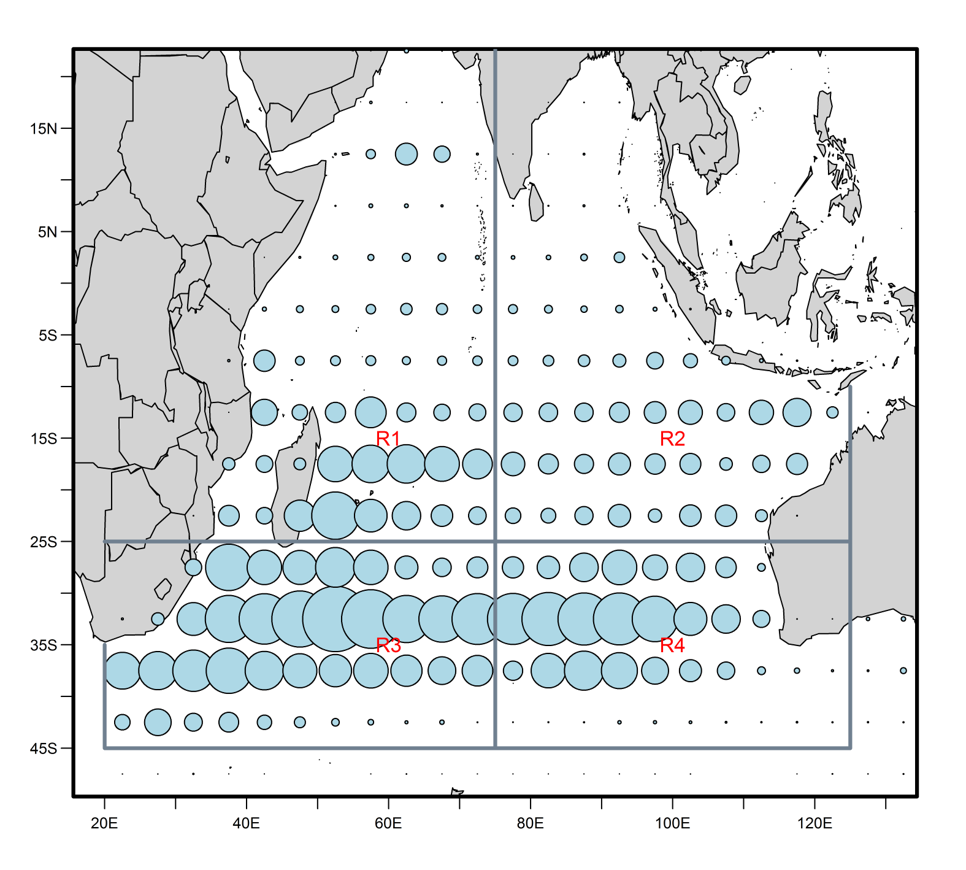
\includegraphics[width=0.75\textwidth]{figures/alb-map.png} 
\caption{Distribution of Indian Ocean albacore tuna catches by assessment areas.}
\label{fig:map}
\end{figure}

\begin{figure}[ht!]\centering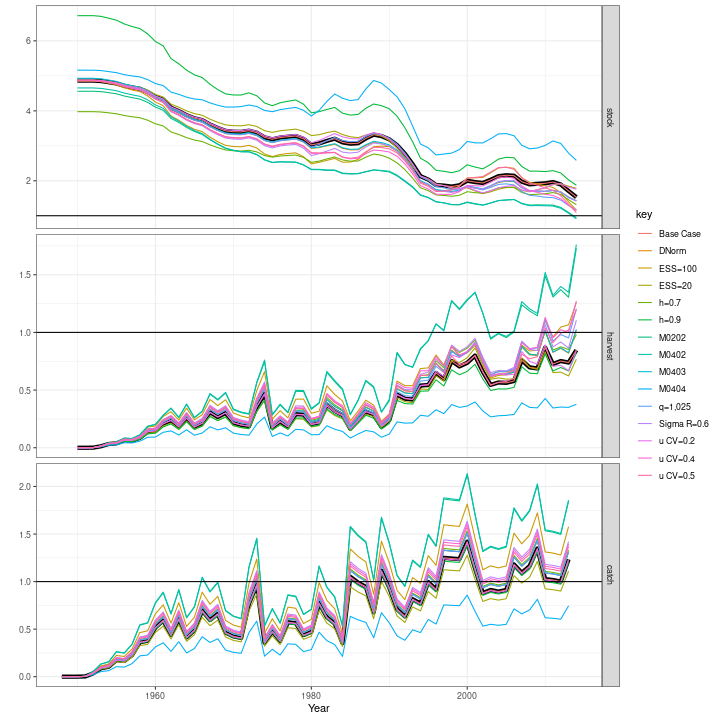
\includegraphics[width=0.75\textwidth]{figures/main-trends-1.png} \caption{Time series of spawning stock biomass and fishing mortality relative to $MSY$ target reference points for the main effects of the Indian Ocean albacore tuna assessment model grid.}
\label{fig:ts}
\end{figure}

\begin{figure}[ht!]\centering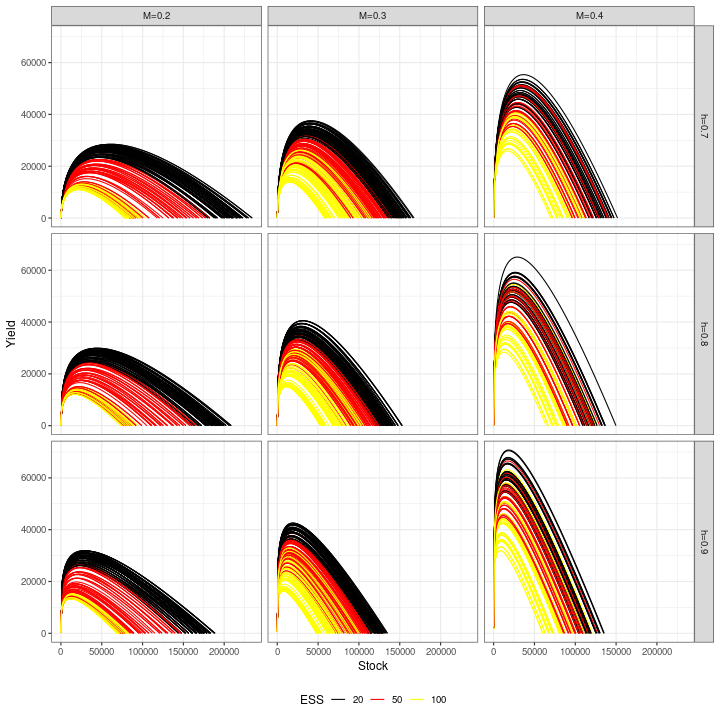
\includegraphics[width=0.75\textwidth]{figures/pf-grid-1.png} 
\caption{Production by steepness and mature natural mortality}
\label{fig:pf}       
\end{figure}

\begin{figure}
        \begin{subfigure}[b]{0.5\textwidth}
               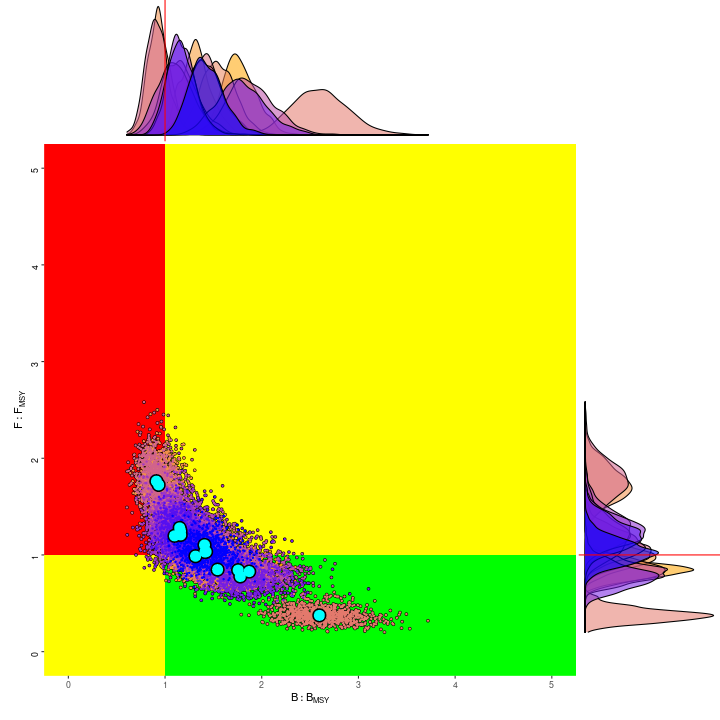
\includegraphics[width=\linewidth]{figures/kobe-main-1.png}
                \caption{Main effects with estimation error.}
                \label{fig:kobe-main}
        \end{subfigure}%
                \begin{subfigure}[b]{0.5\textwidth}
                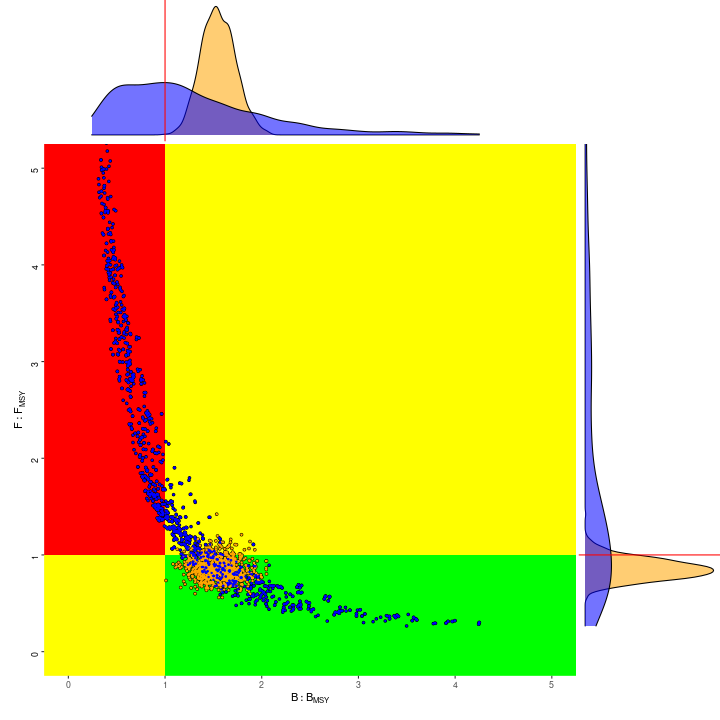
\includegraphics[width=\linewidth]{figures/kobe-bg-1.png}
                \caption{Reference case and grid with model.}
                \label{fig:kobe-bg}
        \end{subfigure}%
        \caption{Kobe phase plots showing spawning biomass ($B$) and fishing mortality ($F$) relative to $MSY$ target reference points. Within model uncertainty was approximating using multivariate log-normal distribution derived from Hessian matrix (MVLN) with cyan points denoting the median}\label{fig:kobe}
\end{figure}

\clearpage
\newpage
\begin{figure}[ht!]\centering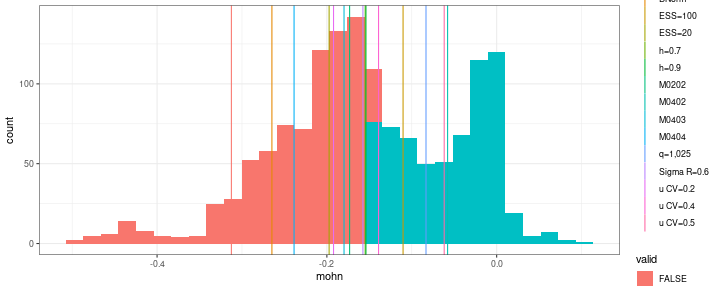
\includegraphics[width=0.75\textwidth]{figures/mohn3-1.png}  \caption{Summary of Mohn's $\rho$ for the for the 1440 assessment models in the Indian Ocean albacore tuna grid, with main effects indicated by the vertical lines.} 
\label{fig:mohn}       
\end{figure}

\begin{figure}
    \begin{subfigure}[a]{0.35\textwidth}
    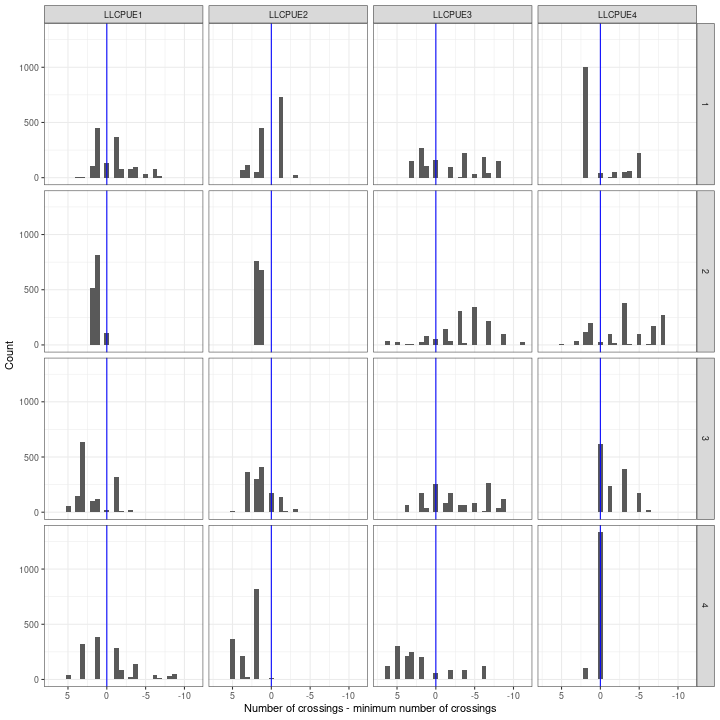
\includegraphics[width=\linewidth]{figures/run-cross-1.png}
    \caption{Number of crossings - minimum expected number of crossings; note reversed x-axis.}
    \label{fig:runs-cross} 
    \end{subfigure}%
    \begin{subfigure}[b]{0.35\textwidth}
    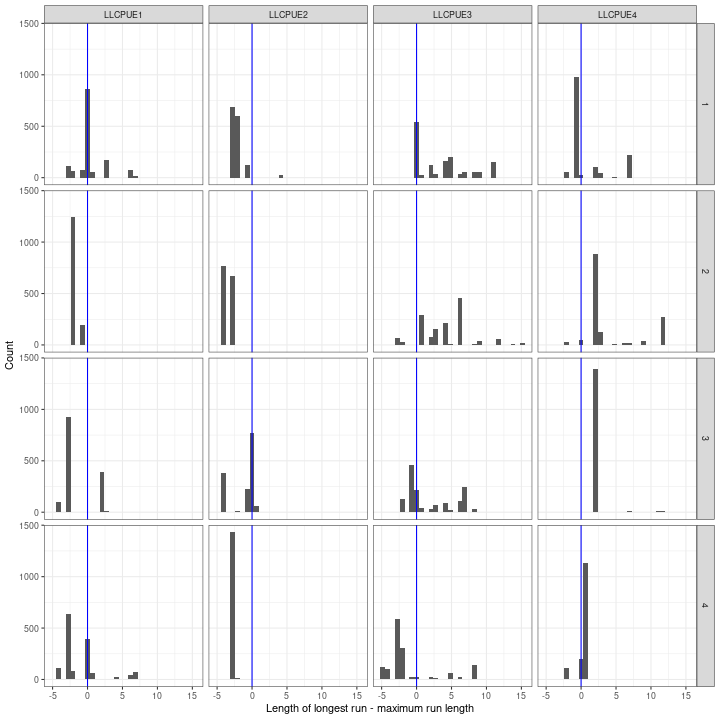
\includegraphics[width=\linewidth]{figures/run-long-1.png}
    \caption{Longest run - maximum expected run length.}
    \label{fig:runs-long}
    \end{subfigure}%
    \begin{subfigure}[c]{0.35\textwidth}
    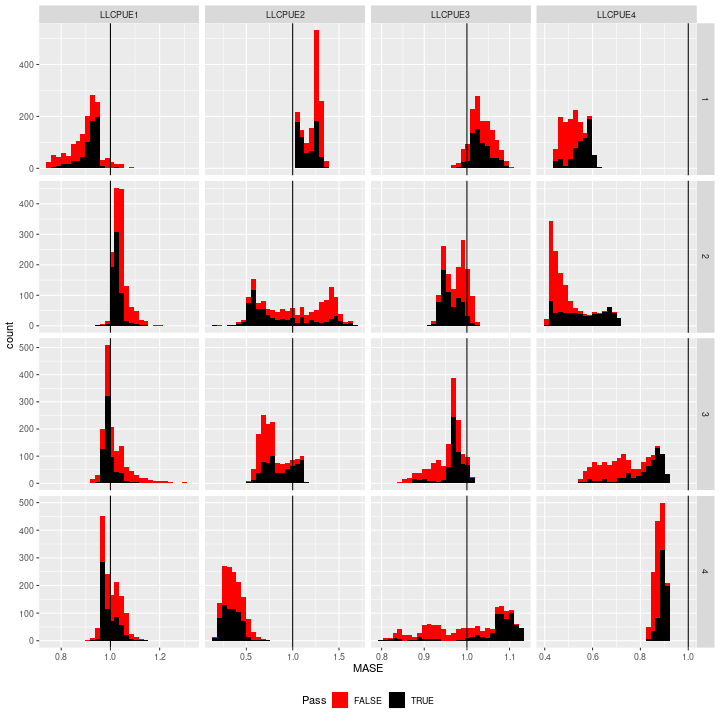
\includegraphics[width=\linewidth]{figures/mase-1.png}
    \caption{MASE.}
    \label{fig:mase}
    \end{subfigure}%
 
\caption{}\label{fig:runs}
\end{figure}


%\begin{figure}[ht!]\centering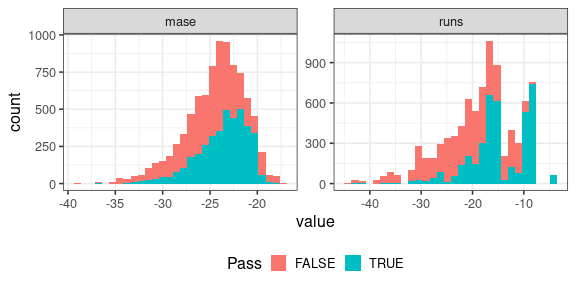
\includegraphics[width=0.75\textwidth]{figures/cf-1.png} \caption{Summary of weighting diagnostics.}\label{fig:wts} \end{figure}

\begin{figure}[ht!]\centering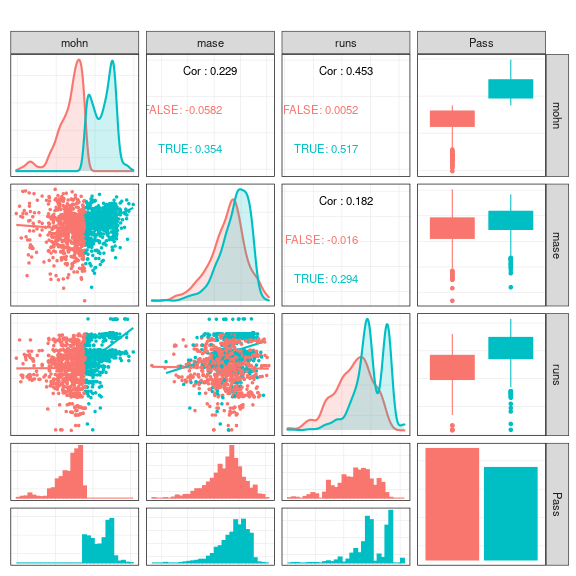
\includegraphics[width=0.75\textwidth]{figures/ggpair-1.png} \caption{Correlations between weighting diagnostics.}
\label{fig:wts}       
\end{figure}

\newpage
\begin{figure}[!ht]
	\centering
	\begin{subfigure}{0.9\textwidth}
		\centering
		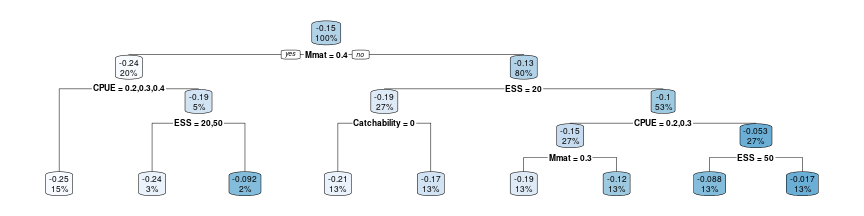
\includegraphics[width=\textwidth]{figures/a-tree-1.png}
		\caption{Regression Tree}
		\label{fig:tree}
	\end{subfigure}
	\hfill
	\begin{subfigure}{0.9\textwidth}  
		\centering 
		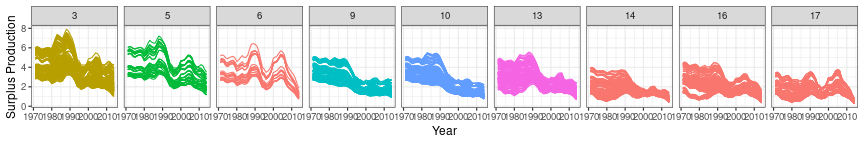
\includegraphics[width=\textwidth]{figures/a-tree-biomass-1.png}
		\caption{SSB}
		\label{fig:tree-b}
	\end{subfigure}
	\begin{subfigure}{0.9\textwidth}  
		\centering 
		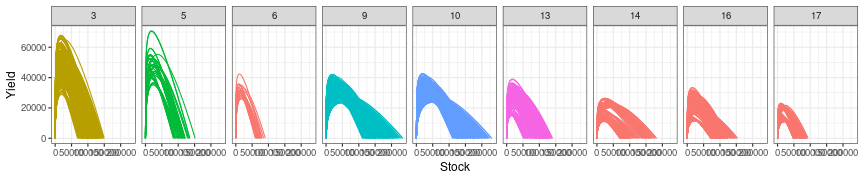
\includegraphics[width=\textwidth]{figures/a-tree-pf-1.png}
		\caption{Production Function}
		\label{fig:tree-pf}
	\end{subfigure}
	\begin{subfigure}{0.9\textwidth}
		\centering
	    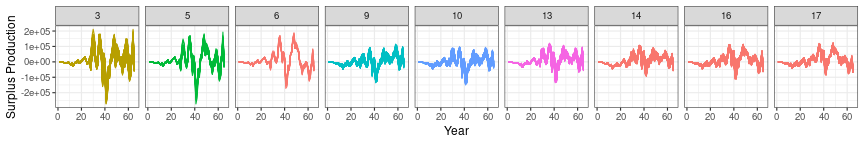
\includegraphics[width=\textwidth]{figures/a-tree-sp-1.png}
		\caption{Surplus Production}
		\label{fig:tree-sp}
	\end{subfigure}
	\caption{Mohn's $\rho$}
	\label{fig:tree}
\end{figure}


\begin{figure}
        \begin{subfigure}[b]{0.5\textwidth}
                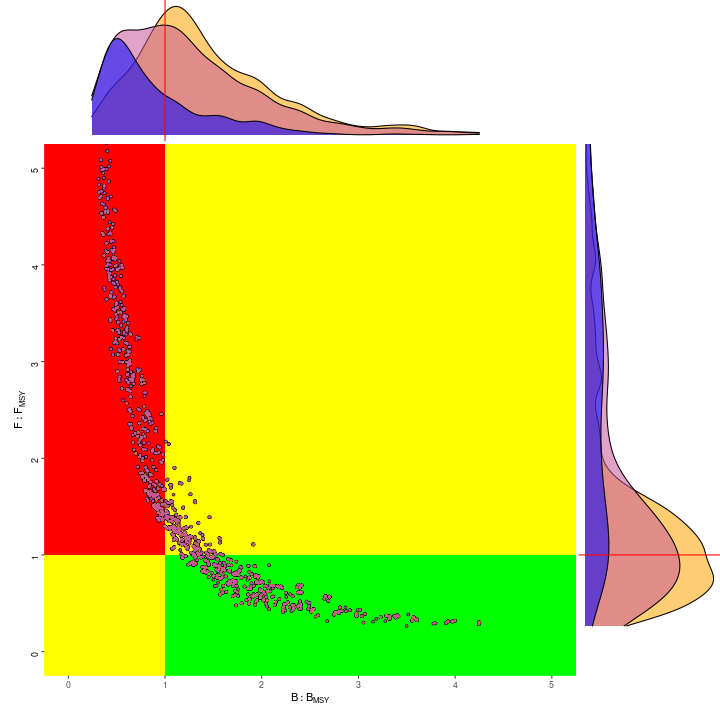
\includegraphics[width=\linewidth]{figures/kobe-mohn3-2.png}
                \caption{Kobe}
                \label{fig:kobe-wt}
        \end{subfigure}%
        \begin{subfigure}[b]{0.5\textwidth}
                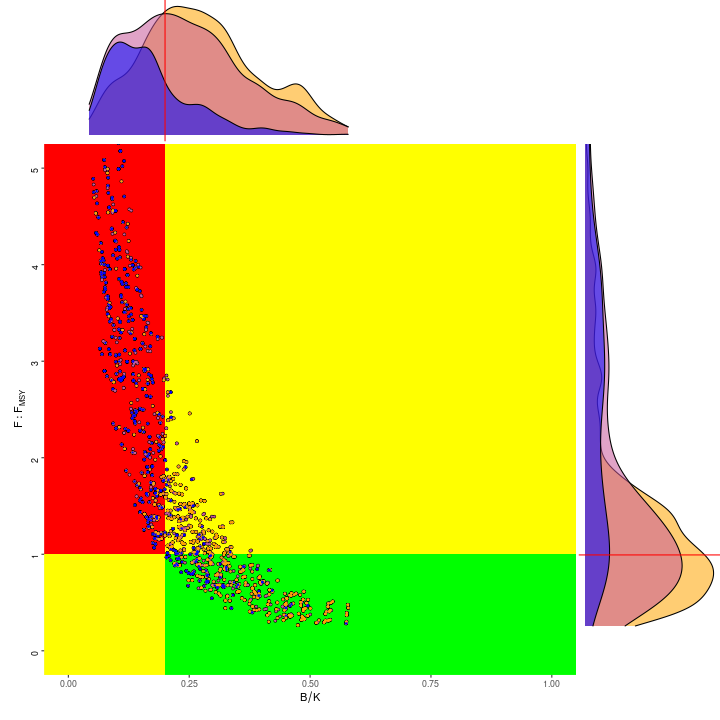
\includegraphics[width=\linewidth]{figures/majuro-mohn3-all-1.png}
                \caption{Majuro}
                \label{fig:majuro-wt}
        \end{subfigure}%
        \caption{Phase plots for all 1440 grid models, with equal, AIC, and skill weighting identifying models that pass the Mohn's $\rho$ test for hindcasts with 3 year ahead forecasts .}
        \label{fig:phase-wt}
\end{figure}


%\begin{figure}[ht!]\centering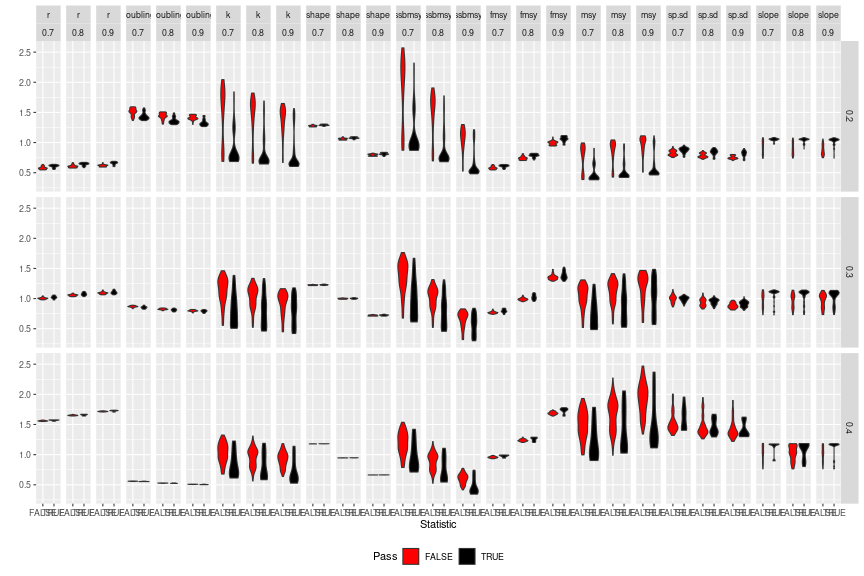
\includegraphics[width=1\textwidth]{figures/param-box-mohn3-1.png}\caption{Summary statistics, will re-do for $F/F_{MSY}$, $B/B_{MSY}$, $r$, $K$, $p$ and $sd(sp)$, and population doubling time.}\label{fig:smry}\end{figure}

\newpage
\begin{figure}[!ht]
	\centering
	\begin{subfigure}{0.32\textwidth}
		\centering
		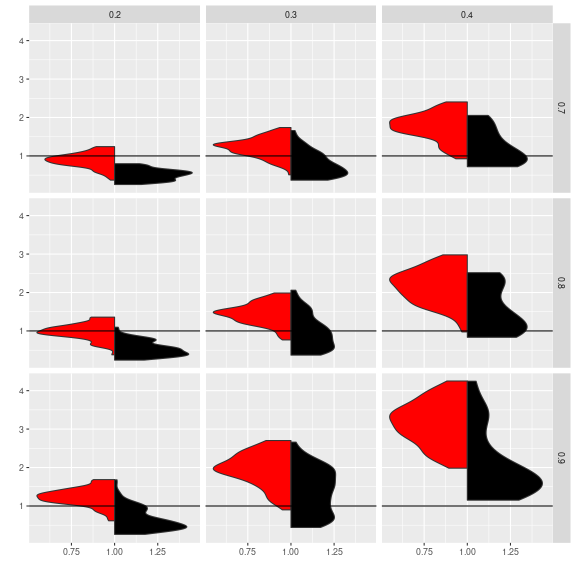
\includegraphics[width=\textwidth]{figures/v-b-1.png}
		\caption{$SSB/B_{MSY}$}
		\label{fig:grid-bmsy}
	\end{subfigure}
	\begin{subfigure}{0.32\textwidth}  
		\centering 
		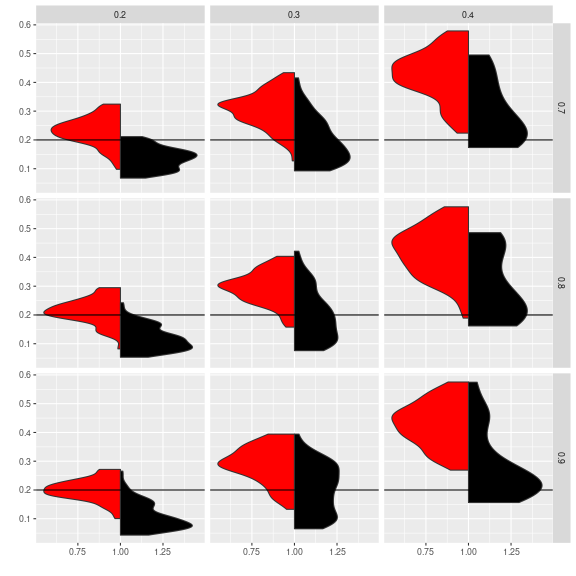
\includegraphics[width=\textwidth]{figures/v-m-1.png}
		\caption{$SSB/K$}
		\label{fig:grid-blim}
	\end{subfigure}
	\begin{subfigure}{0.32\textwidth}  
		\centering 
		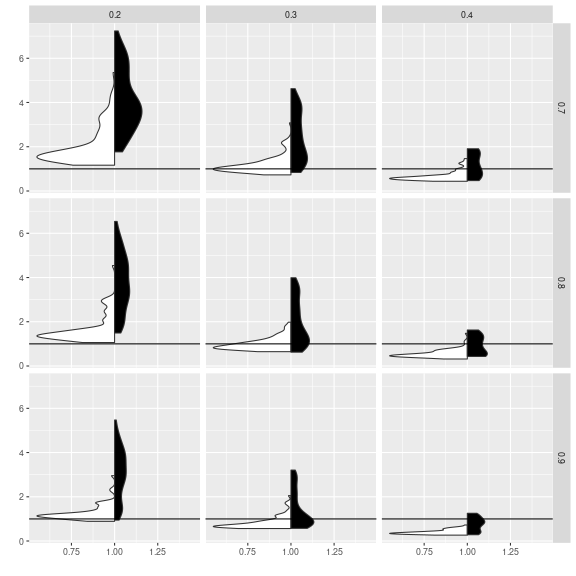
\includegraphics[width=\textwidth]{figures/v-h-1.png}
		\caption{$F/F_{MSY}$}
		\label{fig:grid-fmsy}
	\end{subfigure}
	\begin{subfigure}{0.32\textwidth}  
		\centering 
		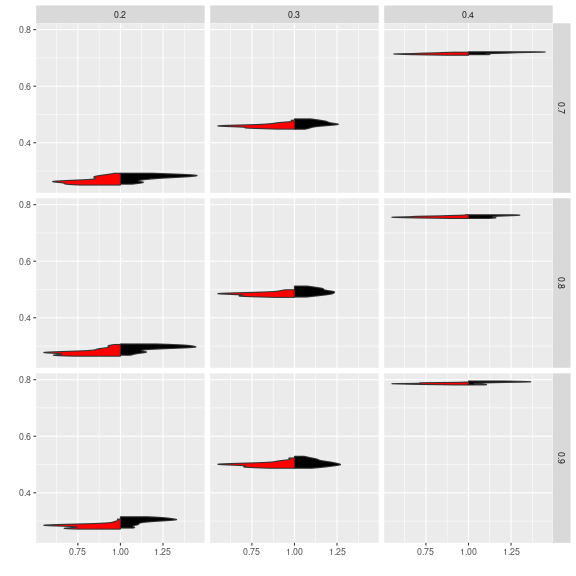
\includegraphics[width=\textwidth]{figures/v-r-1.png}
		\caption{$r$}
		\label{fig:grid-r}
	\end{subfigure}	\begin{subfigure}{0.32\textwidth}  
		\centering 
		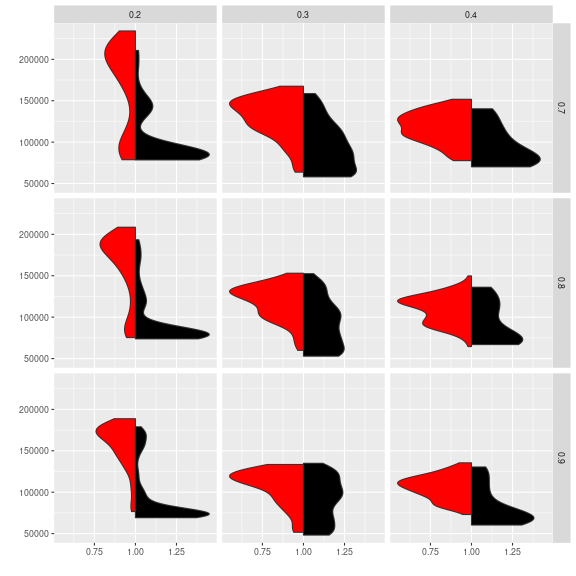
\includegraphics[width=\textwidth]{figures/v-k-1.png}
		\caption{$K$}
		\label{fig:grid-k}
	\end{subfigure}	\begin{subfigure}{0.32\textwidth}  
		\centering 
		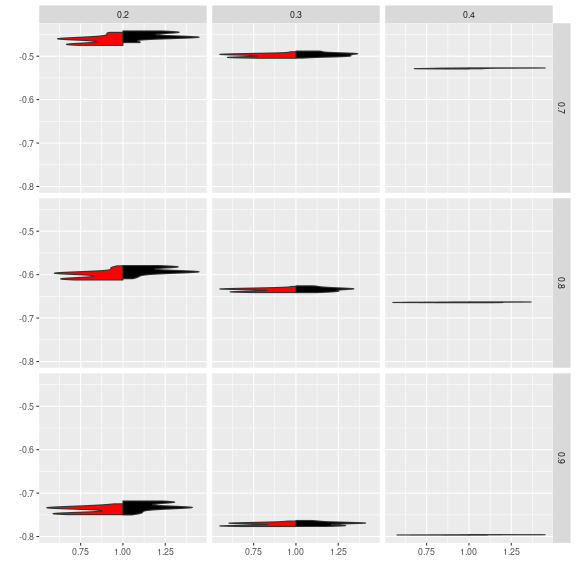
\includegraphics[width=\textwidth]{figures/v-p-1.png}
		\caption{$p$}
		\label{fig:grid-p}
	\end{subfigure}
	\begin{subfigure}{0.32\textwidth}  
		\centering 
		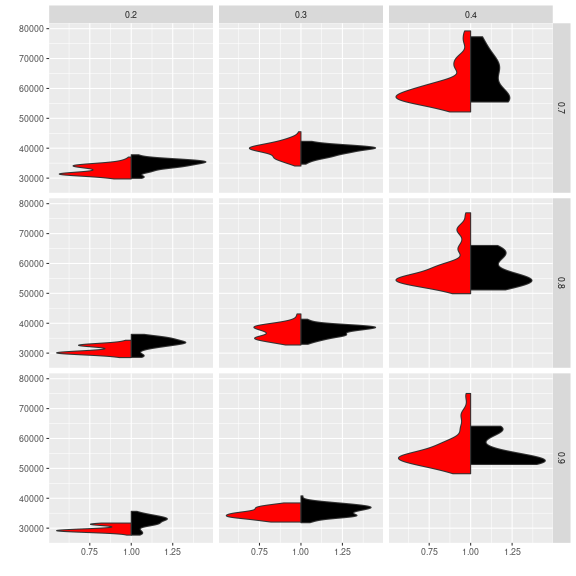
\includegraphics[width=\textwidth]{figures/v-sp-1.png}
		\caption{$sd(sp)$}
		\label{fig:grid-sp}
	\end{subfigure}	\begin{subfigure}{0.32\textwidth}  
		\centering 
		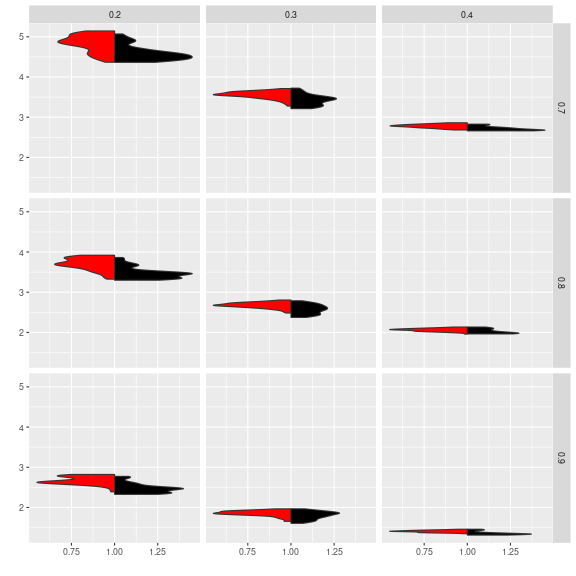
\includegraphics[width=\textwidth]{figures/v-d-1.png}
		\caption{Population doubling time}
		\label{fig:grid-dt}
	\end{subfigure}
	\caption{}
	\label{ref:grid}
\end{figure}

\iffalse
\begin{figure}[ht!]\centering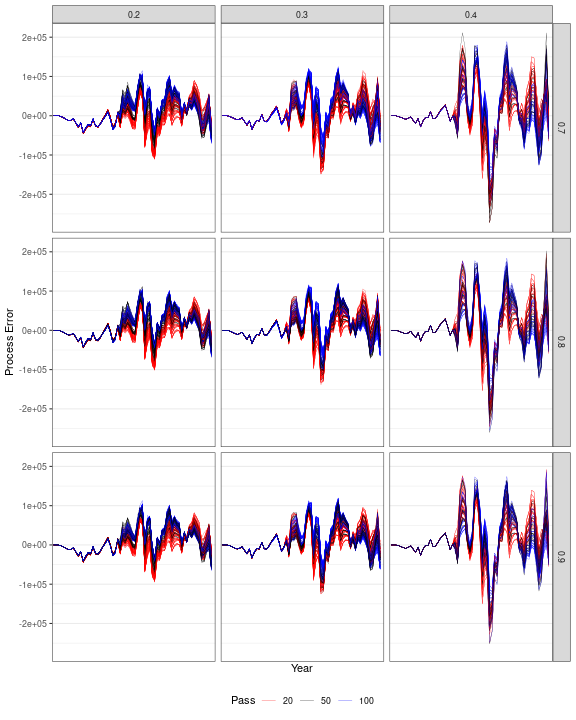
\includegraphics[width=0.75\textwidth]{figures/pf-1.png} 
\caption{Surplus Production by steepness and mature natural mortality}
\label{fig:sp}       
\end{figure}
\fi



\end{document}

\clearpage
\newpage
\section{Tables}

\begin{table}[!ht]
\label{tab:grid}
\caption{Operating Model Scenarios; Base Case values in bold.}  
\begin{center}
\label{tab:datasumm}
\begin{tabular}{|lccc|}
\hline
& {\tiny Levels (N)} & {\tiny $\prod$ N} & {\tiny Values} \\ %& {\tiny Prior} & {\tiny Weighting}\\
\hline\hline
{\tiny Natural mortality (M)& {\tiny 5}}  & {\tiny   5}  & {\tiny  0202  \textbf{0303} 0404 0403 0402}    \\
{\tiny Steepness of the stock-recruitment relationship}}& {\tiny 3} 	 & {\tiny 15}  & {\tiny  \textbf{.7}; 0.8; 0.9} \\
{\tiny Variability of recruitment (sigmaR)}& {\tiny 2} 	 & {\tiny  30}  & {\tiny  \textbf{0.4}; 0.6} \\
{\tiny Effective Sampling Size of the length composition data (ESS)}& {\tiny 3} & {\tiny  90}  & {\tiny  20; \textbf{50}; 100} \\
{\tiny CV for fit to CPUE (cpuecv)}& {\tiny 2} 	 & {\tiny  360}  & {\tiny  0.2;  \textbf{0.3}; 0.4; 0.5} \\
{\tiny Yearly increase in catchability coefficient of CPUE (llq)}& {\tiny 2} 	 & {\tiny   720}  & {\tiny  \textbf{0\%}; 0.25\%} \\
{\tiny Selectivity (llsel)}& {\tiny 2}}& {\tiny 1440}} & {\tiny  \textbf{logistic} double normal} \\
\hline

\end{tabular}
\end{center}
\end{table}

\begin{table}[!ht]
\caption{Mohn's $\rho$ for retrospective analysis.}  
\label{tab:retro}
\centering
\begin{tabular}{rllr}
  \hline
 & run & variable & $\rho$ \\ 
  \hline
  1 & ... & stock & ... \\ 
   \hline
\end{tabular}
\end{table}


\end{document}

\subsection{How to include Figures}

First you have to upload the image file from your computer using the upload link the project menu. Then use the includegraphics command to include it in your document. Use the figure environment and the caption command to add a number and a caption to your figure. See the code for Figure \ref{fig:frog} in this section for an example.

\subsection{How to add Comments}

Comments can be added to your project by clicking on the comment icon in the toolbar above. % * <john.hammersley@gmail.com> 2016-07-03T09:54:16.211Z:
%
% Here's an example comment!
%
To reply to a comment, simply click the reply button in the lower right corner of the comment, and you can close them when you're done.

Comments can also be added to the margins of the compiled PDF using the todo command\todo{Here's a comment in the margin!}, as shown in the example on the right. You can also add inline comments:

\todo[inline, color=green!40]{This is an inline comment.}

\subsection{How to add Tables}

Use the table and tabular commands for basic tables --- see Table~\ref{tab:widgets}, for example. 

\begin{table}
\centering
\begin{tabular}{l|r}
Item & Quantity \\\hline
Widgets & 42 \\
Gadgets & 13
\end{tabular}
\caption{\label{tab:widgets}An example table.}
\end{table}

\subsection{How to write Mathematics}

\LaTeX{} is great at typesetting mathematics. Let $X_1, X_2, \ldots, X_n$ be a sequence of independent and identically distributed random variables with $\text{E}[X_i] = \mu$ and $\text{Var}[X_i] = \sigma^2 < \infty$, and let
\[S_n = \frac{X_1 + X_2 + \cdots + X_n}{n}
      = \frac{1}{n}\sum_{i}^{n} X_i\]
denote their mean. Then as $n$ approaches infinity, the random variables $\sqrt{n}(S_n - \mu)$ converge in distribution to a normal $\mathcal{N}(0, \sigma^2)$.


\subsection{How to create Sections and Subsections}

Use section and subsections to organize your document. Simply use the section and subsection buttons in the toolbar to create them, and we'll handle all the formatting and numbering automatically.

\subsection{How to add Lists}

You can make lists with automatic numbering \dots

\begin{enumerate}
\item Like this,
\item and like this.
\end{enumerate}
\dots or bullet points \dots
\begin{itemize}
\item Like this,
\item and like this.
\end{itemize}

\subsection{How to add Citations and a References List}

You can upload a \verb|.bib| file containing your BibTeX entries, created with JabRef; or import your \href{https://www.overleaf.com/blog/184}{Mendeley}, CiteULike or Zotero library as a \verb|.bib| file. You can then cite entries from it, like this: \cite{greenwade93}. Just remember to specify a bibliography style, as well as the filename of the \verb|.bib|.

You can find a \href{https://www.overleaf.com/help/97-how-to-include-a-bibliography-using-bibtex}{video tutorial here} to learn more about BibTeX.

We hope you find Overleaf useful, and please let us know if you have any feedback using the help menu above --- or use the contact form at \url{https://www.overleaf.com/contact}!








